% Options for packages loaded elsewhere
\PassOptionsToPackage{unicode}{hyperref}
\PassOptionsToPackage{hyphens}{url}
\PassOptionsToPackage{dvipsnames,svgnames*,x11names*}{xcolor}
%
\documentclass[
  brazil,
  a6paper,
  oneside,
  landscape,
  14pt]{scrbook}
\usepackage{lmodern}
\usepackage{amssymb,amsmath}
\usepackage{ifxetex,ifluatex}
\ifnum 0\ifxetex 1\fi\ifluatex 1\fi=0 % if pdftex
  \usepackage[T1]{fontenc}
  \usepackage[utf8]{inputenc}
  \usepackage{textcomp} % provide euro and other symbols
\else % if luatex or xetex
  \usepackage{unicode-math}
  \defaultfontfeatures{Scale=MatchLowercase}
  \defaultfontfeatures[\rmfamily]{Ligatures=TeX,Scale=1}
  \setmainfont[]{Umpush}
\fi
% Use upquote if available, for straight quotes in verbatim environments
\IfFileExists{upquote.sty}{\usepackage{upquote}}{}
\IfFileExists{microtype.sty}{% use microtype if available
  \usepackage[]{microtype}
  \UseMicrotypeSet[protrusion]{basicmath} % disable protrusion for tt fonts
}{}
\makeatletter
\@ifundefined{KOMAClassName}{% if non-KOMA class
  \IfFileExists{parskip.sty}{%
    \usepackage{parskip}
  }{% else
    \setlength{\parindent}{0pt}
    \setlength{\parskip}{6pt plus 2pt minus 1pt}}
}{% if KOMA class
  \KOMAoptions{parskip=half}}
\makeatother
\usepackage{xcolor}
\IfFileExists{xurl.sty}{\usepackage{xurl}}{} % add URL line breaks if available
\IfFileExists{bookmark.sty}{\usepackage{bookmark}}{\usepackage{hyperref}}
\hypersetup{
  pdflang={pt-BR},
  colorlinks=true,
  linkcolor=Maroon,
  filecolor=Maroon,
  citecolor=Blue,
  urlcolor=Blue,
  pdfcreator={LaTeX via pandoc}}
\urlstyle{same} % disable monospaced font for URLs
\usepackage[top=10mm,left=10mm,bottom=10mm,right=10mm,heightrounded]{geometry}
\usepackage{graphicx}
\makeatletter
\def\maxwidth{\ifdim\Gin@nat@width>\linewidth\linewidth\else\Gin@nat@width\fi}
\def\maxheight{\ifdim\Gin@nat@height>\textheight\textheight\else\Gin@nat@height\fi}
\makeatother
% Scale images if necessary, so that they will not overflow the page
% margins by default, and it is still possible to overwrite the defaults
% using explicit options in \includegraphics[width, height, ...]{}
\setkeys{Gin}{width=\maxwidth,height=\maxheight,keepaspectratio}
% Set default figure placement to htbp
\makeatletter
\def\fps@figure{htbp}
\makeatother
\setlength{\emergencystretch}{3em} % prevent overfull lines
\providecommand{\tightlist}{%
  \setlength{\itemsep}{0pt}\setlength{\parskip}{0pt}}
\setcounter{secnumdepth}{-\maxdimen} % remove section numbering
\ifxetex
  % Load polyglossia as late as possible: uses bidi with RTL langages (e.g. Hebrew, Arabic)
  \usepackage{polyglossia}
  \setmainlanguage[]{brazil}
\else
  \usepackage[shorthands=off,main=brazil]{babel}
\fi

\author{}
\date{}

\begin{document}
\frontmatter

\pagestyle{empty}

{
\hypersetup{linkcolor=}
\setcounter{tocdepth}{2}
\tableofcontents
}
\mainmatter
\hypertarget{prefuxe1cio}{%
\chapter*{Prefácio}\label{prefuxe1cio}}
\addcontentsline{toc}{chapter}{Prefácio}

Recebo e organizo todos os textos que foram enviado, mas
\href{https://quarentinestudio.github.io/maria-santana-livro/\#onde-enviar-as-hist\%C3\%B3rias}{continuo
recebendo novos textos}, então caso ainda deseje escrever pode fazer!

Agora estamos entrando na próxima etapa do livro, que consiste em
reunir:

\begin{itemize}
\tightlist
\item
  fotos
\item
  vídeos
\item
  áudios
\item
  desenhos, documentos etc
\end{itemize}

Por favor, enviem para mim o que tiverem sobre vovó que acharem
pertinente, inclusive podem escrever mais sobre a lembrança do item que
estiver enviando (opcional).

Estarei recebendo o material até \textbf{13 de Julho}.

\begin{quote}
\emph{Dudu}.
\end{quote}

\hypertarget{famuxedlia-de-tecla}{%
\chapter{Família de Tecla}\label{famuxedlia-de-tecla}}

\hypertarget{tecla}{%
\section{Tecla}\label{tecla}}

Minha linda e santa Mãe, já faleceu, mas, saudades, dos anos, que viveu
junto a nós.

Desde criança, observei minha mãe, com como uma mulher linda! Tinha
atitudes belas e exemplos! Costumava ir às Missas, muitas vezes, às 4:00
horas da manhã. A Igreja estava sempre lotada. Ela sempre me levava.

Gostava muito de assistir filmes. Era muito vaidosa. Suas vestes ela
comprava tecidos nas lojas Costa \& Júnior, e mandava fazer. Ela tinha
uma mala grande, e nela, mamãe fazia estoque de vestes íntimas.
Costumava ir a salões de beleza. Tinha os cabelos compridos, à altura da
cintura. Quando resolveu cortar, Papai pediu que ela tirasse foto. Esta
fotografia está na sala de Lúcia. Usava cremes no rsto, mas não usava
maquiagem.

Mamãe era muito alegre, gostava de cantar, e aprender algumas notas de
violão. Tinha muitas amigas. As que ela conversava era: Dona
Francisquinha e Penhinha.

Papai nos levava muito para a Praia. Ela gostava de tomar banho de mar.
Nesses passeios, além de nós, filhas e irmã, elava chamava parentes e
amigos para ir junto.

Na nossa casa, sempre tinha hóspedes da família, que vinham de Itabaiana
e de Guarabira.

Com relação a a Educação Escola, mamãe só estudou a Cartilha do ABC.
Minha avó Severina a tirou do colégio para que ela não aprendesse maus
costumes das colegas, por exemplo, dizer palavrões.

No entanto, quando ela conheceu Papai, ambos gostavam muito de ler,
principalmente a Bíblia. Papai comprava inúmeras coleções religiosas e
assinava vários tipos de revistas e tinha livros variados. Essa prática
de leitura ajudou muito na educação.

Lembro que ela dava a papai lindos Cartões Postais com frases de amor.

Quando ela casou com papai, ele teve um desentendimento no trabalho e
ficou sem emprego.

Mas graças a Deus tiveram a ideia de vender bolo e suco na Feira. Mamãe
fazia o bolo e papai fazia os sucos, e vendiam no Mercado.

Com o passar do tempo um amigo de papai emprestou dinheiro para papai
colocar uma Mercearia, assim ele fez. Alugou um local e fez as
prateleiras, comprou algumas mercadorias à prazo. Iniciaram o trabalho.
Ambos sempre foram muito simáticos e logo conseguiram fregueses certos.

Papai contava histórias da Bíblia e alguns livros. Evangelizou muitas
pessoas e os fregueses gostavam.

Na época de Natal e Ano Novo o Bar e a Mercearia ficavam abertos.
Amanhecia o dia e muitas pessoas ainda estavam no Bar e na Mercearia.
\emph{Papai não admitia que os fregueses ficassem nas mesas bebendo},
ele colocava só uma dose de bebida e mandava a pessoa ir dar uma volta.
Vendia mais alimentos e refrigerantes.

Eles contrataram vários empregados, pois eram muitos os fregueses.

A família também foi crescendo. Todos os dias, à hora do almoço, Pai e
Mamãe fechavam o Bar e a Mercearia, para o almoço, que era feito por
mamãe. No próprio local tinha duas salas que ficavam na parte de trás.
Alí mammãe preparava os alimentos e despachava na Mercearia.

Mamãe gostava de gatos, e tinha um loirinho que se chamava Marinheiro.
Era de estimação. Um dia, ele se engasgou com a espinha do peixe e
faleceu, mamãe chorou muito. Nós, os filhos e amigos fizemos o enterro
do gato. Arrumamos uma caixa com flores e enterramos ao lado da @Levada,
que era um Rio bem próximo.

Mamãe gostava muito de andar perfumada, o perfume que ela usava tinha o
nome de Francesa, o pó compacto também tinha o mesmo nome, muito usado
na época.

Mamãe nunca ia a festas. Sempre foi muito caseira e fazia as festas em
casa. Quando havia reuniões festivas na nossa casa Mamãe contratava um
profissional em fazer comidas, que era sua Cmadre e se chamava Natália.

Mamãe gostava de jogar Baralho e semanalmente ela chamava pessoas amigas
pra jogarem. Também começou a jogar o jogo do bicho.

A nossa casa ficava em frente à Praça Getúlio Vargas, na qual ficava a
Igreja e o cinema. Mas duas vezes moramos em duas casas que ficavam na
Rua Juarez Távora. Depois voltamos para a mesma casa que ficava em
frente à mesma praça.

Mamãe fazia pela manhã a Lapa do Padre Rafael. Quando chegava padres
freiras na paróquia era mamãe quem preparava os alimentos. Muitas vezes
ela me mandava arrumar a mesa.

O padre quemais fez refeições na nossa casa foi o Padre João Félix, que
se tornou nosso amigo, que nos visitava sempre mas já está falecido.

Os partos de Mamãe sempre foram feitos pela parteira Dona Isabel. O
parto que ela mais sofrel foi o de Cristina. Ficou um pedaço de gase
dentro de mamãe, e ela teve uma espécie de infecção e foi a Maternidade
Cândida Vargas. Nunca esquieci o olhar triste de mamãe no momento de ir
para a Maternidade. Ela disse para mim: ``\emph{Cuide bem da minha
filha}'' que era a bebezinha.

Os enchovais mais lindos e luxuosos foram os de Cristina e Marta. Todas
nós, irmãs e irmão nascemos em Santa Rita, somente Marta e Feliciano
nasceram em João Pessoa, na maternidade São Vicente de Paulo.

Os anos se passaram, muitas coisas aconteceram. Com o tempo mamãe passou
a ter problemas com a saúde.

Seu estado de saúde se agravou e foi necessário fazer um internamento.

Na última noite que mamãe estava ainda em casa tive a oportunidade de
cantar abraçada a ela. Foi inesquecível este momento.

Passou dias no hospital. Não tive oportunidade de visitá-la nos
primeiros dias, pois havia feito uma cirurgia no pé no mesmo hospital em
que ela estava.

Com a cicatrização do pé chegou o dia de ir visitá-la. Quando a vi com
aqueles maquinários na boca fiquei chocada. Eu disse ``\emph{Mamãe, é
Tecla}''. Ela se ergueu e deitou novamente várias vezes. A minha
impressão é que ela queria falar. Fiquei alguns instantes, terminou o
tempo da visita. Me retirei. Ao chegar na sala em que outras irmãs
esperavam para entrar sentei-me em uma cadeira e as lágrimas vieram aos
olhos e pensei \emph{``Mamãe vai morrer e não a veremos mais.''}

Fui para casa com a minha saudade, consolada pelas orações. Enfim, mamãe
faleceu, deixando para nós lembranças alegres, as ruins procuramos
esquecer\ldots{}

\hypertarget{alexandre}{%
\section{Alexandre}\label{alexandre}}

\hypertarget{adeus-vovuxf3-maria}{%
\subsection{Adeus Vovó Maria}\label{adeus-vovuxf3-maria}}

\textbf{Carta do neto que tanto te ama - 16/05/2007}

Vovó Maria foi vítima das contradições da vida. Soberana na arte de
amar, sucumbiu fiel e majestosamente ao convite do Deus Todo Poderoso de
viver ao seu lado, no Reino da Paz e da Fraternidade. Vovó não fumava,
não bebia, e fugia, o possível, da poluição do meio ambiente, em
passeios matinais pelas ruas dos Bancários, bairro em que morava, onde
ainda, graças as reservas de mata que sobrevivem aos arredores, o ar
resiste ao lixo aéreo da civilização (monstro oculto que cansa e
maltrata o pulmão nosso de cada dia). Impetinente e a mais-que-perfeita
Dona de Casa, tinha para despertá-la, todas as manhãs, o mais singelo
raio solar, os mais belos cânticos de pássaros e o mais apaixonado beijo
do alguém que tanto lhe amou, o seu Pedro.

Vovó representava, incondicionalmente, tudo para nós e, eternamente,
será nossa fonte de carinho, proteção, consolo, ternura, torcida,
conselho e sabedoria. Doutro canto, e por conta disso, havia nela uma
habilidade que me causava ao mesmo tempo profunda admiração e profunda
preocupação, a de estigmatizar-se com a dor e com os problemas de todos
os que a rodeavam. Quem de nós (família), ao menos uma vez, não deitou
no macio e paciente divã da vovó e dividiu com ela um pouquinho da
angústia, frustração, fraqueza ou doença, que nos acometia o momento?
Quem de nós não recorreu a esse tão precioso templo? -- Exemplo de
presteza e doação eu duvido que um dia conheçamos melhor neste palco
existencial.

Mestre da economia do lar, cujas idas aos supermercados e feiras
diplomam sua competência. Ai da despensa! se reclamasse alguma falta
para o almoço do Domingo.

Até nos momentos em que a flagrei triste, sorumbática, tensa,
preocupada, ela me recebeu com sorrisos e demonstrações de perenes
alegrias, como se não houvesse inflação, taxa de juros, perdas no jogo
(Do Bicho), desemprego, corrupção, plano Collor, FMI, mensalão e tudo o
mais que infelicita nossa vida no país. Não! Sobre tal aspecto vovó
sempre foi firme, distante dos problemas. Acho eu, que esse seu
comportamento era uma defesa que usava, uma maneira não violenta de se
opor aos ``Pacotes'' do Governo Federal, à asfixia salarial e mais,
inclusive, um modo seu, peculiar, de resistir às adulteradas contas de
água, luz e telefone, coisas que acontecem para a felicidade dos
mordomos do poder. Sim! Vovó deixou sua contribuição também como cidadã.

Não fui ao hospital. Meu Deus! Nunca me perdoarei por tão grave falta.
Isso porque dias antes da sua internação, percebi, pela doce e singela
expressão de suas feições, que vovó pressentia o fim. Nestes dias ela
andava melancólica, expressando-se pouco, respirando com dificuldade.
Mamãe (Tecla), Tia Lúcia e Tia Dora, também viram, com seus olhos
castanhos, que algo não andava bem em vovó. Eu vi no seu jeito triste,
prenúncios estranhos. Afinal, veio a internação. Na UTI vovó sempre
esteve acompanhada de perto pela equipe médica do hospital UNIMED e pelo
apoio incansável de suas queridas filhas. Não fui lá, mas posso imaginar
tubos e mangueiras lhe envolvendo o corpo, lhe sustentando a vida, lhe
preservando a esperança. Pois como escreveu-nos o Apóstolo Paulo:
\emph{``As tribulações geram perseverança, a perseverança gera
experiência, e a experiência gera esperança''}. Na dimensão de vida
espiritual vovó mais que transcendeu, contudo, neste mundo de aflições e
ainda revestida de corpo corruptível e mortal, de nada adiantaram as
parafernalhas da medicina, pois vovó morreu ontem, dia 15 de Maio de
2007, às 17:00h, num leito frio, de lençóis verdes e tubos brancos
(desculpem-me, minha imaginação insiste em me castigar), próxima aos
braços fortes e morenos de Tia Marta, Tia Bernadete, Tia Dora e Tia
Cristina, vítima de um suspiro letal, que lhe consumiu as últimas forças
de seus bravos pulmões, comprovando sua marca de mulher de fibra e sua
especialidade junto ao divino criador, na pessoa de Pessoa Santa, como
somos todos os que em Cristo descansam.

A morte, às vezes, possui sintomas que levam ao paroxismo, pois a morte
de vovó, ao mesmo tempo em que apunha-la minha alegria, também me enche
de inexplicável contentamento, pois sou fiel na fé que DEUS lhe receberá
de braços abertos e lhe acolherá em glória no paraíso.

Hoje, em nossa família, no aconchego do lar que é de todos nós (a casa
de vovó), existe um vazio de sons, gestos e atitudes, a Rainha do Lar se
foi. Matriarca amada, como dói te perder, principalmente por saber que
igual a ti outra não haverá em nossas vidas, tamanho foi seu amor, sua
fidelidade, sua inteligência, sua bondade, e, sobretudo, SUA
MATERNIDADE.

Assim, por todos nós, amigos e familiares, exalto: - ADEUS MARIA,
INIGUALÁVEL VÓ, FORMIDÁVEL MÃE\ldots{}

E lhe dedico Vó, em nome dos belos filhos que destes ao mundo: José,
Tecla, Lúcia, Lurdinha, Bernadete, Dora, Marta, Cristina e Feliciano
(missionários de seus ensinamentos), essa quadra de um poeta amigo:

\begin{quote}
\emph{``Se um dia me encontrares aqui sozinho e me perguntares o que
vivo planejando assim tão triste e pensativo, Eu te direi que sem te ter
comigo nada existe e sem teu amor não vivo, sobrevivo.''}

-- TEU AMOR ESTARÁ SEMPRE VIVO EM NOSSOS CORAÇÕES!!!

(Teu 1° Neto)
\end{quote}

\hypertarget{tico}{%
\section{Tico}\label{tico}}

Não só eu como muitos eram fãs do \emph{feijão mulatinho} de Dona Maria.
Fui criado tendo como um dos meus hábitos e diversões com mamãe dizendo:
``vamos almoçar na casa da sua vó''. Dito isso, me acostumei a por em
hábito tomar café à tarde com ela, e por muitas vezes também almoçar com
ela.

Sempre fui curioso e adorava ouvir as histórias daquilo que nunca vivi.
Histórias de sua infância, como ela aprendeu o ABC, como conheceu Sr
Pedro, seus passeios às praias de João Pessoa, sua vida em Santa Rita e
etc. Isso para mim tinha um prazer imenso. Não sei dizer o porquê,
apenas era.

Enfim, numa dessas minhas rotinas, certa vez disse a ela que estava com
saudade de comer o seu feijão mulatinho. Ela de pronto me respondeu:
``\emph{sem problemas, meu Neto! Quarta-feira você vem}''. O ano era
2006 e eu estava de férias. Estou eu nesta quarta-feira feira e em casa,
cochilando inclusive. Por coincidência Sr Ailton, que também tinha bons
dotes culinários, havia feito AQUELE feijão também para mim e eu ja
tinha comido uns 3 pratos. O telefone tocou por volta das 13hs. Mamãe me
chama dizendo quer era vovó. Fui atender e vovó na sua voz peculiar me
diz: ``\emph{Tico-Tico, cadê você? Estou com muita fome}''. Minha mente
mesmo sendo boa na hora não me remeteu a nenhum compromisso firmado. Ela
emendou ``\emph{fui na feira e comprei seu feijão, está pronto faz
tempo}''. Eu pensei, ``meu Deus e agora?'' Só pensava nos três pratos
que acabara de comer em casa. Pensei rápido e disse ``Estou lembrado
sim, vovó. Desculpe o atraso mas chego em 10 minutos''. Fui para lá, fui
recebido sempre com seu abraço carinhoso e sentamos à mesa. Ela fazia
maiores louvores de como tinha feito o feijão. Abri a panela e estava
realmente do jeito que fui acostumado a come-lo: bastante jerimum,
rejeito e tudo que tinha direito. Olhei aquele pote de farinha que
ficava numa cumbuca de inox e pensei alto ``\emph{Meu Deus, minha
barriga não cabe mais, porém nao posso desaponta-la}''. Ela me deu
aquele prato de cerâmica muito antigo que tinha um rachão no meio e me
disse ``\emph{está aqui o prato velho que você gosta}''. Confesso que
não sei até hoje onde foi caber esse feijão todo, mas foi muito bom.
Entre uma garfada e outra ela dizia ``\emph{Quer mais}?'' Eu dizia,
``\emph{Claro, vovó! Está muito bom!}'' Conversamos bastante e creio só
ter almoçado no outro dia. Era assim minha relação com Dona Maria.
Aproveitei bastante. Nada é para sempre.

Te amo, Dona Maria! Obrigado por tudo. Do seu neto, Ailton Filho
(\emph{Tico Tico}).

\hypertarget{famuxedlia-de-josuxe9-santana}{%
\chapter{Família de José Santana}\label{famuxedlia-de-josuxe9-santana}}

\hypertarget{janauxedna}{%
\section{Janaína}\label{janauxedna}}

\hypertarget{pequena-mulher-mas-de-uma-vasta-sabedoria}{%
\subsection{Pequena mulher mas de uma vasta
sabedoria}\label{pequena-mulher-mas-de-uma-vasta-sabedoria}}

Maria Santana, minha avó, tivemos poucos momentos juntas, mas foram de
uma riqueza de sabedoria e sentimentos inexplicáveis.~

Nos conhecemos em 2003, quando eu tinha 19 anos, logo após conhecer meu
pai, Dr.~José Santana de Jesus (Duquinha) "``\emph{in memorian}''".

Ele muito entusiasmado em me apresentar para toda a família em João
Pessoa/PB, não contava com as revelações daquela pequena mulher, mas de
uma vasta sabedoria.

Vovó Maria, soube todo tempo da minha existência, porque minha mãe
enviou várias cartas destinadas ao "``\emph{Dr.~Santana}''", meu pai,
entretanto, ela sempre muito reservada, guardava todas as
correspondências, tendo em vista que temia que a esposa dele, na época,
tivesse conhecimento e causasse algum desconforto ou separação do casal.

Assim, como tudo nessa vida tem um propósito, quando tive a oportunidade
de conhecê-la, a primeira reação dela foi ficar arredia, não quis muito
contato comigo, mas em seguida nos mostrou todas as cartas, pediu perdão
por ter escondido do meu pai, mas entendemos que ela fez pela nobre
causa de preservar o matrimônio dele.

Depois desse episódio, tivemos outras oportunidades de estarmos juntas,
ela sempre reservada, mas muito atenciosa, guardo em minha memória as
mais belas recordações de uma mulher de poucas palavras, entretanto,
muito sábia e temente ao Senhor!

\textbf{Janaína Rodrigues Santana de Jesus Oliveira}

\emph{Deus é fiel}!!!

\hypertarget{karlinha}{%
\section{Karlinha}\label{karlinha}}

Olá! Me chamo Karla e sou a primeira neta de vovó Maria, meu convívio
com a vovó infelizmente foi interrompido quando eu era ainda muito
pequena. Então guardo apenas duas lembranças de minha avó com muito
carinho.

A primeira delas, eu era muito pequena não lembro a idade que eu tinha,
morava na torre e lembro de ficar na casa da minha vó olhando o meu avô
preparando, junto com as minhas tias, os bolos para vender na feira e ai
vovó me chamava sempre assim: ``\emph{Karlinha, minha menina, venha
tomar sua vitamina de banana com nescau}''!

E assim que eu pegava o copo ficava demorando a tomar e ela me olhava e
dizia: "\_O que foi você não gosta da vitamina de banana?" E eu super
acanhada falava: ``\emph{Gosto não vovó, vai ficar chateada?}'' Então
ela vinha com leite quente e com açúcar aí eu ameaçava vomitar e aí ela
dizia: ``\emph{Diga pra vovó do que você gosta Karlinha pra eu fazer}''
e ficava me olhando e sorrindo.

E a segunda lembrança é; já adulta fui visitá-la e ela estava na cozinha
fazendo o almoço e algumas das minhas tias a conversar e ela falava
minha gente deixem a menina falar\ldots{} \emph{rsrsrsrs}. Áté porque a
vovó falava pouco, ao menos em minha lembrança, eu a via sorrir mais do
que falar. Então é isso que guardo em meu coração, até que um dia
venhamos a nos encontrar.

\hypertarget{luxfacia}{%
\chapter{Lúcia}\label{luxfacia}}

\hypertarget{histuxf3ria-de-mamuxe3e-maria-josuxe9-de-santana}{%
\section{História de Mamãe -- Maria José de
Santana}\label{histuxf3ria-de-mamuxe3e-maria-josuxe9-de-santana}}

NASCEU EM ITABAIANA, NO DIA 15 DE ABRIL DE 1926. Partiu para o paraíso
no dia 15.05.2007- onde antes falou com Padre Egídio de Carvalho Neto).

SUAS IRMÃS: Maria Augusta (Dáda), Maria Eterna (Madrinha), Maria do
Carmo (Tia Carminha). Seus irmãos: Tio Nezinho -- Tio Olívio -- Tio João
-- Tio Zezinho.

Sua Mãe: Severina Maria de Jesus.

Seu pai: Severino Luiz de Almeida.

Sua Avó: Sebastiana -- seu avô; Manoel Bento - por parte de mãe.

Por parte de pai: João Luiz e Joana.

Se batizou e se Crismou em Itabaiana.

Casou-se com Pedro José de Santana (20.02.1920 - 18.09.2010 -- que
partiu para o paraíso e foi ungido pelo Padre José Carlos serafim) no
dia 15 de outubro de 1943 em Santa Rita Pb, pelo Monsenhor Rafael de
Barros Moreira.

Seus padrinhos de casamento foram: Jucelino F. Mola e Zilda F. Mola.

Entre os convidados estavam: Felícia, Letinha, Zé Maria, Luiz Bento, e
as irmãs!

Teve como filhos:

\begin{enumerate}
\def\labelenumi{\arabic{enumi}.}
\tightlist
\item
  José Santana de Jesus.\footnote{25.07.1944 -- 15.11.2007. Foi ungido
    na hora da morte no dia 20.11.2011 pelo Padre Carlos Maurício!}
\end{enumerate}

\begin{enumerate}
\def\labelenumi{\arabic{enumi}.}
\setcounter{enumi}{1}
\tightlist
\item
  Pedro Santana Filho.\footnote{12.03.1946 e partiu para o paraíso 7
    meses depois.}
\end{enumerate}

\begin{enumerate}
\def\labelenumi{\arabic{enumi}.}
\setcounter{enumi}{2}
\tightlist
\item
  Também teve um aborto espontâneo.\footnote{Seu nome seria João
    Santana, que está no Céu!}
\end{enumerate}

\begin{enumerate}
\def\labelenumi{\arabic{enumi}.}
\setcounter{enumi}{3}
\tightlist
\item
  Tecla Maria de Santana Coutinho.\footnote{Casada com Ailton de Queiroz
    Coutinho.}
\end{enumerate}

\begin{itemize}
\item
  Maria Lúcia de Santana -- Consagrada a Deus em 01.04.1999.
\item
  Maria Bernadete de Santana Medeiros casada com Raimundo da Costa
  Medeiros.
\item
  Maria de Lourdes de Santana Araujo casada com Walter Araujo.
\item
  Maria Marta de Santana Nascimento, casada com Gilberto Nascimento.
\item
  Maria Auxiliadora de Santana Pessoa casada com Jarbas Pessoa.
\item
  Maria Cristina de Santana Freire, casada 2 vezes com Herson Freire.
\item
  Feliciano Santana de Jesus, casado com Marcia Pereira Santana de
  Jesus.
\end{itemize}

As filhas tiveram também netos!

Todos os filhos receberam a Sagrada Comunhão Eucarística:

\begin{itemize}
\item
  Tecla Maria, Lúcia e Bernadete receberam a Comunhão Eucarísitca em
  14.11.1956. Santa Rita.
\item
  José Santana de Jesus recebeu a Comunhão Eucarísitca em 08.12.1952.
\item
  Feliciano recebeu a Sagrada Comunhão Eucarística em 19.11.1977 no
  COLÉGIO Pio X.
\end{itemize}

Datas extraordinárias para o casal Pedro e Maria:

15.10.1978 -- Bodas de Prata.\\
15.10.1993 -- Bodas de Ouro.\\
15.10.2003 -- Bodas de Diamante.

\hypertarget{lencinho-branco}{%
\section{Lencinho branco}\label{lencinho-branco}}

Quando se viram pela primeira vez em João Pessoa, perto da Igreja da
Misericórdia, na esquina! Mamãe acena com um lencinho branco para papai!

Mamãe também disse: todos os dias são de alegria! E quando madrinha
Sebastiana me chamava para vê Pedro passar! -- Mariaaaaa! Vem vê!

Papai disse que sempre está alegre! Quando seus filhos nasceram!

Na Páscoa de 2007 ela disse , quando lhe perguntaram o que era a Páscoa:
\emph{Páscoa é a morte e Ressurreição de Jesus! Ele Ressuscitou e está
vivo no meio de nós! Ele está vivo no meio de nós, por isso é que é
festa! (sorrindo!)}

\hypertarget{rotina-de-mamuxe3e}{%
\section{Rotina de mamãe}\label{rotina-de-mamuxe3e}}

Todos os finais de semana, sexta ou sábado, íamos para a feira no
Mercado Central! Tinha o menino que olhava o carro que ela dava um
dinheirinho! Quando entrávamos no mercado, tinha o senhor que vendia
inhame! Ela conversava muito com ele sobre a família dele e dela! Depois
íamos comprar com a mulher que vendia frango! Novamente parava e
conversava muito com ela! Depois parava no rapaz que vendia carne, que
era Evangélico, e eles conversavam muito sobre a Bíblia! Comprávamos o
resto das coisas e víamos para casa! Ela dizia que eles eram os seus
amigos!

Quando chegávamos em casa, eu, cansada, queria me deitar um pouco, e ela
me chamava para cuidar das coisas! Ia diretamente para a cozinha!
Gostava de lê a Bíblia, os Salmos! Um dia ouviu alguém dizer: Leia o
Deuteronômio ! Ela disse que leu por obediência, mas não entendeu nada!

Gostava também de jogar bicho, que era para ajudar um filho ou outro e
também para se distrair! Quando os filhos estavam com problemas
financeiros ou de qualquer natureza, sofria muito!

Todos os dias rezava o Terço! Também assistia Canção Nova, que gostava
muito! Ela dizia que a Canção Nova a ajudou na sua vida Cristã! Escreveu
para Luzia Santiago por duas vezes e ela respondeu!

Ela ajudava muito os pobres, assim como papai! Tinha uma senhora, D.
Joana, que vinha aqui com o seu neto, um adolescente! E mamãe a mandava
entrar! Colocava comida para ela, a ouvia, e lhe dava uma feirinha!
Quando soube que D. Zefinha estava passando fome, começamos a levar uma
feira para ela! E mamãe e Odete, uma amiga de mamãe, andaram no INSS, e
em vários lugares para aposentar D. Zefinha e até que conseguiram!

Odete recebia também a Palavra de Vida, que falava de uma Leira Bíblica!
Odete foi quem descobriu a Canção Nova e nos disse para ligar! Uma
grande amiga!

\hypertarget{caudados-e-orientauxe7uxe3o-com-os-filhos}{%
\section{Caudados e orientação com os
filhos}\label{caudados-e-orientauxe7uxe3o-com-os-filhos}}

Quando comecei a estudar na Escola Técnica, Mamãe fez questão de me
levar com papai! Naquela época eu tinha problemas de depressão, e ficava
feliz com a ajuda de papai e mamãe! Mamãe foi uma pessoa que nos amava
muito, muito cuidado com todas nós! Nos orientava, para que não
caíssemos em nada errado! Eu sempre disse que Mamãe era como São José,
uma pessoa justa! Agradeço muito a Deus por me ter dado mamãe como minha
mãe!

Não a amei tanto como ela merecia! Uma vez, eu estava aborrecida, e fui
saindo com o carro, e, sem querer, ia dá ré no carro e fui para frente e
bati nela! Pedi muito perdão a Deus! Ela ficou muito sentida! Ás vezes
ela ficava sentada na cozinha e eu sentava junto a ela! Sempre ela
conversava dos filhos que ela achava o grande tesouro! Houve um tempo em
que os filhos vinham almoçar aqui em nossa casa! Ela ficava muito feliz
em fazer aquela comida tão gostosa!

Todos os Domingos íamos para a Missa na Torre, e tomávamos café na casa
de Madrinha Eterna! Lembro bem, cuscuz com carne guisada! Madrinha
Eterna foi quem ajudou a mamãe a se aposentar! Ela pagava todos os meses
o carnê de mamãe pois mamãe não ia no banco! Agradeço a Deus, Madrinha
Eterna e Dáda, que sempre estavam nas nossas festinhas! Mamãe era muito
unida com elas e tia Carminha! Depois Madrinha Eterna ficou doente, e
foi encolhendo! Dorinha a sobrinha, filha de tia Carminha foi quem
cuidou dela! E Dáda veio aqui para nossa casa! Embora eu cuidasse de
Dáda, Mamãe se sentia responsável por ela! E ela dizia: \emph{Não tenho
condições de cuidar de Augusta! E falou para a irmã cuidar}! Gracinha,
filha de Tia Carminha decidiu cuidar de Dáda!

Mamãe é uma pessoa maravilhosa! Sabe pedir perdão, se desculpar!

\begin{quote}
-- Querida mamãe, obrigada! Deus em nós faz este milagre! DEUS EM NÓS
NOS FAZ PERDOAR TODOS os sofrimentos!
\end{quote}

\begin{quote}
-- MAMÃE, obrigada por me ter criado, por me ter educado, por ter me
alimentado, por ter se preocupado com o nosso estudo!
\end{quote}

Lembro, que saiu de Santa Rita para procurar uma casa em João Pessoa,
pois pensava na frente! Naquele tempo, não tinha estudo em Santa Rita! E
o maior desejo de nossa mãe, era que estudássemos! \emph{Obrigada,
mamãe}!

Nos colocou em Colégios em João Pessoa! Estudei com Bernadete no Colégio
Lins de Vasconcelos, um Colégio muito Conceituado, e Tecla estudou no
Colégio Getúlio Vargas! Depois saiu com D. Zefinha, procurando casa para
que morássemos em João Pessoa!

Naquele tempo, as finanças estavam em decadência! Mas Mamãe teve Fé,
acreditou que daria certo! Encontrou uma casa no Bairro de Jaguaribe, na
Rua Professor Renato Carneiro da Cunha! Ali, começamos a comer um
pirãozinho que Mamãe fazia: farinha, cebola, coentro! Uma delícia! Papai
sem dinheiro para pagar o aluguel da casa, foi quando começamos a
trabalhar! Primeiro Tecla e Bernadete! Depois eu trabalhei na Padaria
Santo Antonio, na Rua Alberto de Brito!

Eu comprava pão nesta padaria, e um dia, Diana, a caixa da padaria, me
disse: -- Lúcia, vou sair da padaria! E gostaria que você trabalhasse no
meu lugar! Então eu disse: -- vou falar com mamãe! Chegando em casa,
disse a mamãe que Diana tinha me chamado para trabalhar na Padaria!
Mamãe, então disse: -- \emph{vá minha filha}! Uma semana depois, Diana
me chamou. Tirei a minha carteira de Trabalho ainda de menor! Tinha 17
anos! O primeiro salário, que foi 10,00. Dei a mamãe! E ela pediu para
comprar carne e outros alimentos! Quanta alegria foi naquele dia!

Agradeço a mamãe, que pedia para nós mesmos, fôssemos no Colégio, para
nos matricular! Eu era muito tímida, e Tecla e Bernadete tomavam a
frente! Mas Mamãe estava sempre nos orientando! Mamãe dia para que
fôssemos para a Missa todos os Domingos!

Então, um dia, papai se ajoelhou e pediu a Deus, um trabalho para
alimentar a família! E ele disse que \emph{Deus inspirou para ele fazer
bolo}! Ele fez um bolo, vendeu todo, trouxe o dinheiro e materiais para
fazer mais! Então, todas as irmãs e Feliciano, fazíamos bolo, e mamãe
ficava com a alimentação! Então foram momentos muito bons, podemos pagar
todas as despesas e aluguel da casa! Papai chegava em casa com um
presente para mamãe: era um tecido, uma sandália, flores\ldots{} ela
ficava muito feliz!

Cada vez mais eles eram mais unidos! Todos os Domingos fazia almoço para
todos os filhos e noras e genros! Foi quando também nos mudamos para
outra casa no Bairro da Torre. Lá tivemos dificuldades, meu irmão queria
que ficássemos numa casa, que a justiça estava pedindo! Mamãe teve a
iniciativa de sairmos daquela casa! Berna antes, tinha alugado essa
outra casa! Passado esta dificuldade, moramos nesta outra casa que tinha
um quintal grande, onde fazíamos o bolo!

Lembro das galinhas correndo atrás da gente! Eu tinha muito medo! Eu
ficava mais para limpar a casa! Lembro que a casa tinha um pé de fruta
pão! Mas não comíamos! Feliciano precisava fazer uma cirurgia! Ainda
morávamos na casa anterior, eu tinha passado no concurso do Banco,
Bernadete também tinha passado no concurso do Banco, e quando eu fui
chamada para trabalhar,\footnote{Nessa época, eu estava trabalhando no
  Tribunal de Contas.} Mamãe estava em São Paulo, pois Feliciano foi
fazer a cirurgia da garganta em São Paulo! Quando disse a mamãe que
tinha sido chamada para trabalhar no Banco, ela disse: \emph{só viaje
quando eu voltar}! E também papai estava com saudade de mamãe! Cantou
para ela: ``recebe as flores que te dou'' Então mamãe chegou e eu dei
entrada nos papéis para viajar!

Enquanto estava em Breves, eu ligava para ela e ela perguntava como eu
estava! Quando cheguei em Breves pela primeira vez, não sabia onde tinha
telefone, nada! Passei uma semana sem dar notícias! Mamãe sofreu muito!
Depois Gracinha minha prima, conseguiu falar com uma casa de madeira que
tinha na cidade de Breves, e soube notícias minhas! Eu era muito
desorientada! Depois de 1 ano, nove meses e 25 dias, voltei para João
Pessoa!

\hypertarget{o-movimento-dos-focolares-entre-nuxf3s}{%
\section{O Movimento dos Focolares entre
nós}\label{o-movimento-dos-focolares-entre-nuxf3s}}

Minha mãe se preocupava muito comigo! Passei uns três anos morando em
Goiana PE! Depois voltei! Foi quando conheci o Movimento dos Focolares!
Foi uma transformação na minha vida! Saia muito o dia todo para entregar
a Palavra de Vida, e ela ficava preocupada! Uma vez á noite, um carro me
seguiu, e não saí mais à noite! Ela pensava que eu iria deixá-la pelo
Movimento dos Focolares, e ficava preocupada! E eu, também desorientada,
não dizia nada a ela, ficava calada! Eu tinha um Amor muito grande pelo
Movimento dos Focolares, mas tinha muitas dúvidas! Foi quando em
01.05.1999 eu me Consagrei a Deus! O Padre disse que eu iria renovar a
Consagração a cada 4 meses! E ainda faço isto! Falei com Mamãe e ela
ficou muito triste! Mas não disse nada! E eu também fiquei calada! Era
doente, tomava remédios controlados!

Quando comecei a estudar, Duquinho me levava com ele para a faculdade!
Quando nos formamos, depois, eu e Berna fomos estudar na Escola, um
curso de Turismo e Mamãe e Papai ia me levar e buscar em Jaguaribe! Não
lembro porque, Berna ficou separada de mim.

Então, eu e mamãe conversávamos muito, levava ela em Dr.~Aécio,
psiquiatra, que ela gostava muito! Eles conversavam muito! Ela era como
uma mãe para Dr.~Aécio! Também Dr.ª Sandra! Quando se encontravam se
abraçavam e conversavam muito! Eu ficava sempre calada! Também Mamãe ia
para Dr.ª Elsie e também conversavam muito!

\hypertarget{a-partida}{%
\section{A partida}\label{a-partida}}

Como disse anteriormente, conversava muito com suas irmãs, mas depois
elas faleceram e ela ficou muito triste! Dizia: \emph{Meu filhos são o
meu tesouro}! Ela sofria de problemas respiratórios e sempre usava
aquela bombinha! Íamos para o mercado todas as sextas ou sábados, até
aquele dia que foi o último dia em que ela foi para feira, na sexta
feira! Chegou em casa, ajeitou a comida e depois ficou doente! Chamei
Berna que veio imediatamente! Levou ela para o hospital! Passou uns
dias, e voltou e disse que \emph{tinha sentido a minha falta no hospital
para acompanhá-la}! Depois, Padre Egídio veio aqui, e conversou com ela!
Ela estava na cozinha! Ficou feliz quando viu Padre Egídio, mas depois,
fechou os olhos e ficou assim\ldots{}

Berna falou novamente com Dra Sandra e ela disse que a levasse para o
hospital, que ficou com um respiradouro! Depois piorou e a entubaram,
passaram uns dias, fui visitá-la, sofri muito vê-la naquele estado, pois
me lembrei que ela tinha uma dor nos queixos, e naquele momento estava
com um tubo na boca! Sofri muito! E depois ela partiu!

Duquinho, penso, foi quem mais sofreu com a partida de mamãe! Ela
cuidava dele, o ouvia\ldots{} Agora ela é um Anjo! Está numa outra
dimensão! Está com Deus! Está feliz! Está com a Virgem Maria, com Jesus,
com a Corte Celeste!

\hypertarget{famuxedlia-de-bernadete}{%
\chapter{Família de Bernadete}\label{famuxedlia-de-bernadete}}

\hypertarget{bernadete}{%
\section{Bernadete}\label{bernadete}}

\hypertarget{eu-e-mamuxe3e}{%
\subsection{Eu e mamãe}\label{eu-e-mamuxe3e}}

Minha mãe!!! O que falar dela? Amorosa, dedicada aos filhos, Esposa
exemplar! Envergonhada, tímida, Forte como um touro.

Me lembro eu pequenininha sentada em cima de uma mesa em nossa casa em
Santa Rita-PB e mamãe fazendo bolinhos de feijão verde no meu prato e
colocando para eu comer. Ela tinha que misturar tudo pois só assim eu
comia. Também das vezes que eu ia com ela na levada (uma espécie de rio
pequeno e estreito), pois ela lavava a roupa de nossa casa, e lá eu
ficava em cima de uma pedra pegando os peixinhos pequeninos que passava
e logo eu caia de cara na água e mamãe, muito assustada, corria para me
segurar com medo que eu morresse afogada.

Mamãe junto com papai eram muito cuidadosos com a nossa religião, e
lembro que mamãe me acordava as 5 horas de manhã para assistir a missa
no domingo. Eu acordava e ficava com preguiça de me arrumar e mamãe com
a maior paciência me dava banho vestia a minha roupa e penteava os meus
cabelos. Eu tinha o cabelo grande e batia na cintura como não gostava
muito de pentear ele ficava todo embaraçado e mamãe com o pente
lentamente escovava todas as mechas.

Logo cedo eu fui estudar no colégio Santa Verônica e mamãe era muito
cuidadosa engomava a minha farda que era toda plinssada e fazia uma
saias de baixo com vários bicos e eu andava toda chique. Com sapatos bem
limpos de verniz preto e meias com pompons de lado.

Aos cinco anos eu fiz a minha primeira comunhão com minhas irmãs Tecla e
Lúcia. Mamãe contratou uma costureira para fazer os nossos vestidos ela
teve todo um cuidado. Nosso vestido era de organdi branco liso e
estampado tinha várias saias por baixo meu livrinho era branco com o
retrato de Jesus na capa, o terço de prata, havia uma coroa com véu
branco na cabeça. Nós parecíamos mais umas noivas e mamãe feliz da vida
nos levou para receber Jesus na praça Getúlio Vargas, onde o bispo deu a
eucaristia para mais de 100 crianças. Neste dia eu perdi o meu lanche
que eu havia recebido do colégio e chorei muito. Eu estava doente havia
me recuperado de bexiga e mamãe com a maior paciência me consolou e
disse que quando chegasse em casa faria outro lanche para mim.

Fomos crescendo e mamãe sempre atenta aos que nos acontecia. Durante o
ano havia as festas de Natal, Ano novo, Festa de Reis e o São João e
mamãe muito precavida pois tinha muitos filhos sempre vinha para João
Pessoa e comprava tecidos para fazer nossos vestidos, roupas de cama e
cortinas para nossa casa. Eu era sempre quem a acompanhava nesta viagens
e ela ia para as Casas Costa Junior e lá ela tinha alguns vendedores que
já a conhecia e separava alguns tecidos para ela. Após fazer as compras
e enquanto o funcionário tirava as notas nós íamos assistir filme no
Cinema Brasil que ficava ao lado da loja eram filmes de Mazaropi, Eliana
e Oscarito, Derci Gonçalves, La Violetera (Com Sarita Montiel), Dio como
te amo, etc. O que eu mais gostava era que quando saíamos do filme ela
ia comigo ao bar em frente do edifício do Ipase e nós comíamos caldo de
cana com bolo e pão doce.

Eu gostava muito de ficar vendo tudo o que mamãe fazia e ia para a
cozinha com ela para ver ela fazer a comida e sempre escutava aquela
frase de que eu não gostava ``Lugar da criança não é na cozinha''. Eu
ficava triste pois queria ver como se cozinhava, mas para me consolar
ela deixava eu ficar embaixo da mesa brincando com as minhas bonecas e
fazendo sofá e mesa com caixas de fósforo. Eu passava horas ali pertinho
da minha mãe pois, eu via as pernas dela enquanto estava em pé junto à
mesa e me sentia segura.

Uma das coisas que eu não gostava em mamãe era que ela sempre que ia
brigar comigo me dava uns cocorotes e também uns beliscões na perna e
isso doía muito então eu não gostava. As vezes eu levava a culpa por
coisas que eu não havia feito e eu achava isso uma injustiça. Quando
isto acontecia eu passava uma semana sem olhar na cara de mamãe e ela
dizia olhe para mim menina e eu ficava de cabeça baixo pois tinha
vergonha de ser chamada a atenção.

Papai tinha um bar, uma mercearia e um bar de caldo de cana e mamãe
ajudava ele nos trabalhos. Eu como sempre muito metida estava sempre lá
junto de mamãe. Uma coisa que eu adorava a fazer era o doce de banana.
Mamãe trazia as bananas que estavam maduras de mercearia e que não
tinham sido vendidas para fazer doce então, mamãe colocava as bananas no
tacho e eu ficava muito feliz por que ela me deixava amassar as bananas
com minhas mãos (Só após lavá-las) e eu ficava ali toda orgulhosa por
que estava ajudando. Também ela me ensinou a lavar os copos e me
colocava em cima de um tamborete e eu alcançava a pia e então lavava os
copos e ela guardava.

Também ela fazia almoço para os motoristas de ônibus que freqüentavam o
nosso bar, ela colocava no prato arroz, tomate, alface e um bife de
carne ou de frango com suco de vários tipos como maracujá, coco,
mangaba, cajá, uva, laranja, caju etc. E eu aproveitava para ajudar
levando as garrafas de suco para colocar na geladeira. Era uma geladeira
de 8 portas que ficava cheinha de garrafas de suco.

Nas festas de Ano novo se vendia muitos bolos e queijo do reino na
mercearia e no bar. Mamãe e papai colocavam mesas na frente do bar para
servir as pessoas e mamãe ficava com agente a noite toda servindo. Ela
muito cuidadosa colocava papai para dormir pois ele não gostava quando
chegava um bêbado e ficava enchendo a paciência então mamãe ia lá e
consertava as coisas.

Essas festas eram muito animadas. Nós vestíamos vestidos e sapatos novos
e cada pessoa queria mostrar o seu novo modelo de festa. Logo à tardinha
mamãe me arrumava junto com minhas irmãs e nos colocava sentadas na
porta de casa para ver as pessoas passarem. Muita gente passava para
conversar conosco e algumas queriam ver a minha roupa olhavam até as
minhas calcinhas eu chorava e ia dizer a mamãe.

Fui crescendo e mamãe sempre cuidadosa para que nós tivéssemos uma boa
educação e fossemos prendadas ela me colocou para aprender bordados na
máquina e fazer bainhas na mão, me colocou na aula de artes e eu fui
aprendendo muitas coisas. Acho que é por isso que hoje gosto tanto de
artesanato e crochê, ponto de cruz, costurar etc. Tudo isso era amor ela
queria suas filhas bem preparadas para enfrentar o futuro o emprego e o
casamento.

Havia também o mês de maio e em nossa Paróquia eram feitos os novenários
durante todos os trinta e um dias do mês. A imagem de Nossa Senhora
visitava 31 casas na cidade e uma delas era a nossa. Este momento era
esperado com muita ansiedade. Mamãe tinha um carinho especial por Nossa
Senhora e ela preparava a charola (andor onde se leva as imagens sacras
nas procissões) com muito carinho. Eu ia com mamãe no comércio para
comprar tecidos para envolver o andor. Mamãe escolhia os mais bonitos e
brilhantes. Lembro de um em que ela fez uma lua aos pés de Nossa Senhora
e o tecido era todo brilhoso e na cor prata então todos os que olhavam
ficavam admirados com tanta beleza. Ela contratava uma Senhora de nome
Dona Cotinha que era uma artista e ela com muito carinho preparava tudo.

Á tardinha mamãe nos vestia com roupas de Anjo e nós ficávamos na
calçada sentadas na cadeira esperando a hora de ir para a procissão.
Lembro que eu gostava muito destes momentos, mamãe permitia que nós
puséssemos batom e rouge . Todos queriam ver o dia da nossa procissão
porque era a mais comentada do mês. Papai comprava velas e dava para
todas as pessoas e era um belo cortejo. Na Igreja papai e mamãe sentavam
juntos e nós os anjinhos ficávamos em cima do altar. O momento mais belo
que eu achava era quando se cantava a Ladainha e quando o Pe. Incensava
o altar.

Por um período por que Lúcia estava doente de coqueluche moramos um
tempo na Praia do Bessa e mamãe ficava muito preocupada pois por causa
do trabalho ela e papai ficavam em Santa Rita e nós ficávamos com as
empregadas na praia. A nossa maior alegria era quando ela chegava com
papai nos finais de semana.

Cresci e mamãe com papai nos colocaram para estudar no Lins de
Vasconcelos em João Pessoa pois mamãe queria que nos tivéssemos o melhor
estudo para se formar e conseguir um bom emprego por que eles não
puderam estudar. Mamãe e papai tiveram uma decepção com o colégio das
Neves pois lá só conseguiam vaga os pais das crianças que tivessem muito
dinheiro e nós não fomos aceitas lá.

Lembro que mamãe era muito preocupada com o meu irmão Santana que dava
muito trabalho a ela. Ele tinha uma namorada e aos 15 anos comprou todos
os utensílios para a casa da namorada e disse que ia casar. Mamãe ficou
muito preocupada pois ele não tinha emprego e ela ficava procurando ele
nos lugares em que estava com a namorada e mandava ele para casa. Todas
as vezes que papai brigava com ele por causa de namorada ele fugia de
casa e vinha para João Pessoa para a casa de tia Carminha só após mamãe
chorar muito e procurar ele era que ele vinha para casa. Antes nós as
irmãs pensávamos que mamãe não gostava das filhas pois ele só se
preocupava com o seu filho Santana mas depois com o tempo nós fomos
crescendo e entendendo que não era falta de amor e sim que os pais se
preocupam mais com os filhos que dão mais trabalho.

Mamãe era romântica gostava muito de ouvir musicas e tinha um gosto
diversificado. Lembro das músicas mexicanas, das de violão com
Dilermando Reis, de Dalva de Oliveira,Trio Iraquitam Roberto Leal e
canções como Beija-me muito, Aqueles olhos verdes, Fascinação, Três
Palavras (Como te quero) etc. Também era uma ótima cozinheira fazia
pratos deliciosos a sua carne de panela é lembrada até hoje pelos seus
filhos e o três em um de sobremesa quase ninguém sabe fazer com o
gostinho que ela preparava. Nós fazemos, mas, não fazemos igual.

Com o tempo já com oito filhos os negócios de papai deram para trás e
mamãe ficou muito triste já não podia comprar dois vestidos para cada
uma nas festas, não podíamos comprar sapatos, até a comida ficou
escassa. Papai ficou sem opção e mudou-se para João Pessoa para ver se
melhorava de vida. Um dia ele não tinha nem o dinheiro para pagar o
aluguel e o dono da casa chamou papai de velhaco. Então papai pediu a
Deus que lhe desse uma luz. ``O que ele poderia fazer para poder criar a
sua família'' e lhe veio à idéia de fazer o bolo e vender nos bares e
mercearias. Neste período mamãe ficou grávida do seu último filho
Feliciano. Ela sofreu muito não tinha plano de saúde então papai fez
para ela um INSS de trabalhador autônomo como costureira e ela pôde ir
para a maternidade. Feliciano chegou em um momento muito difícil mamãe
chorava todos os dias ela não tinha dinheiro para fazer os lençóis, as
camisas e as fraldas dele então, eu havia aprendido a fazer umas
sandálias de ráfia e fiz algumas sandálias vendi as minhas amigas e
comprei o tecido para fazer o enxoval de Feliciano. Mamãe ficou muito
feliz e ela cortou as camisinhas os lençóis e as fraldas e eu costurei e
fiz as camisinhas à mão. Ela me ensinou um ponto bem pequeninho (Bainha)
que se faz nas camisas de bebê e nós juntas ficamos muitos felizes.

Após este episódio eu e Lúcia saímos e conseguimos emprego. Lúcia em uma
padaria e, todo dia ela trazia o pão para casa e entregava para mamãe e
eu no escritório de uma casa de tecidos e todo o meu dinheiro que
recebia dava a ela. Foi um período muito bom. Nós mudamos de casa fomos
morar na Alberto de Brito e tudo voltou a melhorar. Mamãe estava feliz
novamente.

O tempo passou e começaram os namoros. Mamãe sempre muito atenta a nós
para que não ficássemos moças faladas e ela sempre nos alertava para ter
cuidado com os namorados. Na Alberto de Brito eu comecei a namorar com
Raimundo.

Após um tempo nos mudamos para a Torre e fomos morar na Severino
Patrício. Mamãe estava feliz com a nova casa. Nós não iríamos pagar
aluguel, pois a casa pertencia ao nosso irmão Santana que nesta época já
havia casado.

Nesta casa nós fomos felizes. Tinha uma sala grande e como eram muitas
pessoas nós forrávamos o chão da sala e dormíamos ali. E era uma
algazarra total e mamãe sempre nos dizia ``Meninas olha o silêncio vamos
dormir''. Depois mamãe encomendou para Tecla um enxoval, pois ela estava
namorando Ailton e mamãe como sempre e cuidadosa com as filhas preparou
tudo. Tecla foi a única filha que teve o enxoval preparado por mamãe.
Depois veio o casamento de Tecla e logo após o meu. Mamãe ficou muito
preocupada com meu casamento, pois nesta época eu dava todo o meu
salário a ela e eu saindo de casa iria fazer falta, mas, conversei com
Raimundo e ficamos dando uma parte a ela e graças a Deus nunca nos
faltou nada.

Mas nesta casa mamãe teve também um grande desgosto. Vejam só teve
alegria na entrada e desgosto na saída. A casa do meu irmão foi para
leilão da Caixa e tivemos que sair de lá às pressas para não sermos
despejados. Quem mais sofreu neste caso foi mamãe, pois ela acreditava
que eles não viriam fazer o despejo mais eles vieram e mamãe sofreu uma
grande vergonha.

Neste período eu tinha ido trabalhar em São Paulo e como já havia
voltado estava na casa de mamãe procurando uma casa para morar. Como
aconteceu isto e eu havia alugado uma casa para morar na Miguel Santa
Cruz da Torre então chamei mamãe para morar comigo. Como ela não tinha
opção e foi despejada ela foi morar comigo.

Nesta casa casaram Cristina, Auxiliadora e Marta. Para mamãe foi um
grande baque aquela casa antes cheia de gente estava se esvaziando. Ela
não conseguia pensar que as meninas não mais estariam em casa. Como toda
a mãe ela queria que nós sempre estivéssemos sob a sua proteção como a
galinha com seus pintinhos.

Após um período fui morar no bairro dos bancários e mamãe ficou
novamente sem mais uma de suas filhas. Chegando lá eu Lúcia e Ailton
pensamos em conseguir uma casa para mamãe morar junto a nós e compramos
a chave de uma casa perto da minha. Foi uma grande alegria mamãe
novamente ia morar em uma casa dela e sem pagar aluguel.

Nesta casa mamãe teve muitas alegrias e sofrimentos mais o importante
era que estava junto dos seus. Aos poucos minhas irmãs foram vindo morar
em casas perto a ela e elas levava seus filhos para ficar com mamãe para
poderem trabalhar.

Mamãe estava novamente educando. Os netos ficavam com mamãe. Uns o dia
todo e outros apenas um período. Mamãe se dividia em cuidar deles e
fazer o bolo. Nesta época a fábrica de bolos havia crescido e todos os
dias eram muitos bolos. Papai vendia na vizinhança e todos ficavam
felizes. Era um bolo muito gostoso. Mamãe tinha muitos ajudantes mais a
responsabilidade total era dela de tudo sair em ordem. Ela ficava
cansada à noite de tanto tirar o botar as assadeiras no forno durante
todo o dia.

Havia uma coisa que mamãe gostava muito era o seu jogo do bicho. Ela
ficava entretida fazendo seus jogos e milhares. Sonhava e logo dizia
qual será o bicho?. Perguntava a todos o que você sonhou hoje? Ela
queria ter um palpite. Quando ela assistia um filme ou uma novela na
televisão ela logo anotava o número das placas dos carros. Gostava muito
de Silvio Santo. Vivia sonhando de um dia acertar na Telesena. Mais o
que ela mais queria era com esse dinheiro poder ajudar aos filhos e
noras para que nenhum passasse dificuldades. Sempre que sabia que algum
estava em dificuldades logo chegava lá e procurava resolver aquele
problema. Mamãe ajudou a muita gente era muito generosa.

Mamãe era muito envergonhada e ficava com vergonha quando papai abraça e
beijava ela e sempre dizia ``Sai Pedro''. Ela tinha vergonha de abraçar
até as filhas. Eu aprendi com papai e sempre que chegava eu dava um
abraço nela. De início ele não abraçava mas com o tempo quando agente
chegava perto ela ia logo dando os braços para abraçar. Mamãe era muito
linda era muito elegante. Gostava de usar cremes, sapatos novos,
sabonete (Alma de Flores) perfume Alfazema, cinta, meias finas, vestidos
novos, cintos, etc. Também gostava de comprar louças de porcelana e
pratos de vidro decorados. Quando nós éramos pequenas abríamos uma mala
que mamãe tinha e vestíamos as roupas, sapatos e meias de mamãe quando
ela descobria o que nós fazíamos nos colocava de castigo sentadas no
chão por uma hora.

Mamãe era muito amorosa sempre que fazia galinha ela guardava a moela
para mim. Quando eu chegava ela dizia ``olhe que guardei para você''.
nas festas de São João fazia canjica e pamonha e guardava sempre uma
pamonha e um prato de canjica para cada filho. Me pedia sempre para
organizar a festa de aniversário de cada filho ou filha e nos domingos
gostava sempre de almoçar com todos os filhos juntos. Ela gostava de
fazer pirão de carne e sempre me pedia para eu mexer o pirão com ela e
eu ficava muito contente por estes momentos de intimidade.

Todos os Natais nós estávamos juntos. Fazíamos amigo secreto, papai
Noel, árvore de Natal e muita comida que era dividida por todos. A nossa
vida era uma festa e mamãe não queria perder nenhuma.

Nossa casa era cheia de pessoas que vinham para papai rezar de mau
olhado e outras enfermidades e mamãe na maior paciência acolhia a todos
que chegavam.

Todos os domingos ia para a missa com papai, gostava de rezar o terço e
o Ofício de Nossa Senhora. Um dia minha mãe teve uma gripe e dessa gripe
foi para o hospital passando 15 dias interna lá. Fiquei com ela durante
estes quinze dias e visitava 3 vezes por dia mas mamãe não resistiu e
partiu para o paraíso.

Tenho muita saudades da minha mãe mas, sei que Deus precisou dela e ela
teve que partir. Sei que agora ela é um anjo do céu e que fez toda a sua
parte quando estava conosco.

Teria muitas coisas para falar da minha mãe mas, vou dar oportunidade de
minhas irmãs falarem algo mais.

\begin{quote}
\emph{Bernadete}
\end{quote}

\hypertarget{dudu}{%
\section{Dudu}\label{dudu}}

\hypertarget{vovuxf3-maria}{%
\subsection{Vovó Maria}\label{vovuxf3-maria}}

Vovó Maria, é assim que me refiro a ela.

A gente vinha na casa de vovó

\begin{itemize}
\tightlist
\item
  almoço de feliciano
\end{itemize}

\hypertarget{sala-cozinha-e-comida}{%
\subsection{Sala, cozinha e comida}\label{sala-cozinha-e-comida}}

Como neto, a presença de vovó costumava está associada a \emph{cozinha},
\emph{sala}, \emph{família} e \emph{comida}.

Como gordinho que eu \emph{era}, a casa de vovó tinha uma atração: uma
boboniere em formato de casinha, aquilo me encantava.

\hypertarget{reencontro}{%
\subsection{Reencontro}\label{reencontro}}

Na época, eu estava casado e morando fora da casa dos meus pais. Vovô já
tinha falecido há poucos anos.

Lá em casa, a gente costumava realizar ``O evangelho no
lar'',\footnote{Trata-se de um encontro semanal, sendo previamente
  marcado o dia e a hora, (devendo ser repetido sempre no mesmo dia e
  hora da semana) com o objetivo de reunir a família em torno dos
  ensinamentos evangélicos, à luz do Espiritismo, e sob a assistência
  dos Benfeitores Espirituais.} uma reunião espírita entre os
familiares, realizados na residência, com textos edificantes para
reflexão -- um compromisso semanal em que mentores espirituais costumam
trazer espíritos que irão se beneficiar das mensagens que serão
abordadas.

Nesta noite, Paty encontrava-se lá em casa, e ao aproximar-se o horário
da reunião foi convidada a participar também.

Durante a reunião, um espírito se aproximou e pediu para pegar na mão de
Paty e depois na minha.

O espírito era vovó, que ainda encontrava por aqui. Durante a reunião
\emph{ela conseguiu enxergar vovô}, e se reencontravam novamente.
Ocasião em que relatou que ele (vovô) estava \emph{mais novo}.

Mamãe e Patrícia costumavam relatar sentir a presença de vovó na casa
delas, mas somente após esse evento veio a certeza, no meio coração, de
que vovó se rencontrou com vovô e eles estão bem no além.

\hypertarget{paty}{%
\section{Paty}\label{paty}}

\hypertarget{o-que-dizer-da-vovuxf3-maria}{%
\subsection{O que dizer da ``vovó
Maria''?}\label{o-que-dizer-da-vovuxf3-maria}}

Cabelos brancos, macios e com cheirinho de bebê, sorriso lindo
envergonhado. Chegávamos na casa dela e podíamos encontrá-la geralmente
sentadinha na mesa da cozinha com seu bom e velho caderninho de
anotações. O Vesper (telefone sem fio) estava sempre ao lado, e o almoço
ou a janta no fogo. Os netos eram recebidos sempre com um chocolate e um
sorriso. Ela sempre tinha algo para nos dá.

Lembrar de vovó é lembrar dos almoços de domingos, das festas, da
aglomeração dos fins de semana. Um almoço não era apenas um almoço, era
um evento onde comparecia cerca de 30 pessoas, entre filhos, netos e
agregados. Um coração gigantesco e sempre pronto a ajudar. Uma das suas
especialidades era ``escutar'', todos chegavam com seus problemas e ela
escutava, sem julgamentos. Sob um manto de fragilidade, ela era uma
mulher forte, guerreira. Lembro que um dia algo aconteceu que tive que
ir ao Mercado Central com ela fazer as compras. Era fim de semana e isso
era sinônimo de muitas pessoas. Ela chegou com sua roupinha de compras:
saia longa abaixo do joelho, uma blusa, seu sapatinho de compras e sua
bolsinha. Saímos do carro e me deparei com milhares de pessoas e uma
confusão de vozes. Vendo aquilo, me coloquei prontamente à frente da
minha avó e fui praticamente abrindo espaço pra ela poder passar, fazia
praticamente uma barreira com os braços para proteger minha vozinha
daqueles transeuntes desatentos que batia um nos outros com a maior
normalidade do mundo. Eu ali, ``achando'' que a estava protegendo
daquelas pessoas, mas a realidade era outra, na verdade, aquelas pessoas
precisavam dela, e ela daquelas pessoas. Após os minutos iniciais
chegamos aos boxes de compras, comecei a observar a desenvoltura com que
ela se misturava ao ambiente. Ela era chamada pelo nome por onde
passava, sabia exatamente onde comprar cada coisa, e onde não comprar,
perguntava se hoje tinha esse ou aquele produto, também chamava as
pessoas pelo nome. Eu achando que estava a ``protegendo'', enquanto que
ela estava ali me dando lições de vida e humildade, ensinava pelo
exemplo. Minha avó era assim, aparentemente frágil, quase angelical, mas
com uma força de leão por dentro, força esta que a ajudou a criar uma
dezena de filhos, netos e bisnetos. Saudades!

\hypertarget{famuxedlia-de-lourdes}{%
\chapter{Família de Lourdes}\label{famuxedlia-de-lourdes}}

\hypertarget{lourdes}{%
\section{Lourdes}\label{lourdes}}

\hypertarget{mamuxe3e-exemplo-de-mulher-esposa-muxe3e-avuxf3-bisavuxf3-amiga}{%
\subsection{Mamãe, Exemplo de Mulher, Esposa, Mãe, Avó, Bisavó,
amiga!}\label{mamuxe3e-exemplo-de-mulher-esposa-muxe3e-avuxf3-bisavuxf3-amiga}}

\textbf{Simplificando: MAMÃE, EXEMPLO DE MULHER CRISTÃ}

\begin{figure}
\centering
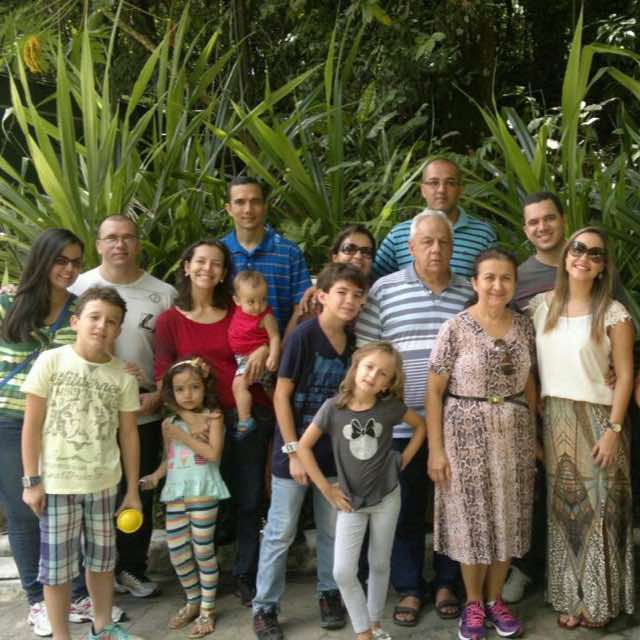
\includegraphics[width=2.90625in,height=2.90625in]{img/lourdes/image1.jpeg}
\caption{MARIA DE LOURDES SANTANA DE ARAÚJO, Casada com Walter de
Araújo, Filhos: \textbf{Fábio Augusto Santana de Araújo}, (casado com
Kelma Silva de Araújo -- Filhos: Fábio Lucas Silva de Araújo e Karine
Silva de Araújo), \textbf{Walber Santana de Araújo}, (Casado com Aline
Kelly dos Santos Santana de Araújo -- Filhos: Isabelle dos Santos
Santana de Araújo e Iago dos Santos Santana de Araújo), \textbf{Wagner
Santana de Araújo} (Casado com Elziellen Hêmilie Evangelista de Araújo
-- Filho: Arthur Wolfgang Nóbrega de Araújo) e \textbf{Walter Santana de
Araújo}, casado com Sheila Luna de Luna de Santana.}
\end{figure}

Agradeço a Deus pela infância que tive ao lado dos meus irmãos, e irmãs.
Agradeço a Deus por ter nascido e crescido num lar ajustado. Apesar de
ser a filha do meio, fui criada com mimos, como também minhas demais
irmãs.

Nasci em uma família onde o amor prevalecia. Meus pais nos deram exemplo
na simplicidade deles, do valor da família, trabalho, honestidade,
integridade, temor à Deus. Cresci vendo minha mãe trabalhando. Mamãe, um
exemplo de mulher, esposa, mãe. Falava pouco, sempre tímida, o sorriso
dela era lindo! Cabelo lindo, arrumado e tratado. Ela usava no cabelo um
creme Kolene, Pó promessa no rosto, Cache mire Bouquet, Creme Ponds C,
para limpeza de pele, Colônia alfazema. Quando papai tinha a Mercearia e
o Bar, ela passava o dia lá, ajudava bastante papai. Ficava na cozinha,
lavava a louça e fazia comidas deliciosas. Nós fazíamos as refeições na
Mercearia. Não me lembro de ter apanhado de mamãe, (apesar de ter
merecido) mas lembro de que certa vez ela correu atrás de mim com uma
chinela na mão e eu me acabando de rir porque ela não me pegava!

Como eu era criança não sei quantas vezes mamãe arrumou a charola onde
colocavam a imagem que era levada em uma procissão. Ela nos vestia de
anjo, eu e minha irmã Marta, para irmos à frente da imagem durante a
procissão.

Certa vez, eu estava brincando de pega-pega, folhinha verde - e correndo
descalça, pisei em um pedaço de vidro, saiu muito sangue e mamãe me
levou na farmácia. Colocaram uma gaze no meu pé e fiquei andando com um
pé só. Em outra brincadeira brincando de boneca, esbarrei em uma porta
de madeira que tinha vidro. Ela caiu em cima de mim, coloquei a mão para
evitar a pancada, furou minha mão e meu braço, lá vai minha mãe me
socorrendo levando para a Farmácia, lembro que a dona da Farmácia era
minha xará, chamava-se Dona Lourdes. Mamãe me contou de como escapei
duas vezes de morrer; uma de CRUPE, doença infecciosa que pode matar com
24 hrs, se não tiver uma assistência imediata. E a outra de morrer
AFOGADA. O medico havia recomendado para ela me dar banho de mar, eu
estava com manchas na pele. E na inocência dela, foi me dar banho
estando à maré alta. Uma onda me arrebatou dos braços dela, e alguém,
``acredito um anjo'', me pegou e me entregou nos braços dela! Lembro da
primeira vez que fiquei sabendo da minha idade. Ela estava diante do
espelho penteando o cabelo e eu perguntei: - Mamãe, quantos anos eu
tenho? E quando eu nasci? Ela me respondeu: - Você tem 7 anos! Você
nasceu em 21 dezembro de 1954! Dalí em diante fiquei acompanhando ano a
ano a data do meu aniversário! Quando menstruei a primeira vez, lembro
que ela estava lavando louça, abri a porta do banheiro e mostrei para
ela! Ela saiu da cozinha e voltou com uns paninhos na mão e me disse: -
É assim, vai acontecer todo mês, use esses paninhos, lave e guarde para
usar quando precisar. Pronto, simples e prático! Risos\ldots{} Primeira
e ultima vez que conversamos sobre esse assunto.

Cozinhava excelentemente bem! Feijoada deliciosa! Peixe, Cosido de
carne, galinha assada! Ainda hoje Walter meu esposo comenta: Até hoje,
nunca comi uma galinha assada como Dona Maria fazia! E muito mais
comidas saborosas! Aprendemos a fazer a famosa sobremesa que ela fazia:
chamávamos ``Três cores'' ou ``Manjar do Céu''. Passa de geração a
geração! Netos e bisnetos amam!

Quando eu queria alguma coisa e ela não deixava eu ficava insistindo até
ela deixar! Risos\ldots{} Porque eu só queria fazer com o consentimento
dela. Se eu fosse brincar na casa de uma amiga ela dizia a hora de
voltar e eu procurava voltar na hora combinada, para que ela deixasse
que eu fosse novamente. Lembro que minhas irmãs mais velhas diziam que
eu conquistava mamãe e ela fazia o que eu queria. Quando elas queriam
sair para algum canto me pediam para eu falar com mamãe, porque eu
sempre conseguia convencê-la!.

Quando chegou o tempo de fazermos o bolo baêta, enquanto estávamos
fazendo o bolo, mamãe ficava na cozinha preparando as refeições e
lavando a louça. Ela quem nos servia, colocava a comida no prato de cada
filho! No final de semana fazíamos a faxina, cada uma tinha uma tarefa,
inclusive de lavar a louça. Mamãe gostava de jogar no bicho e estava
sempre querendo saber o que tínhamos sonhado para jogar.

Crescemos ouvindo papai chamar mamãe de; minha namorada, minha
queridinha, minha flor\ldots{} Que lindo! Quando ele chegava da rua
depois que vendia os bolos, costumava trazer algo para ela; sandália,
corte de tecido, e até o alimento e ele dizia: -- Maria! Queridinha!
Presente minha filha! Que lindo! São lembranças lindas deixadas pelos
nossos queridos pais! Quando papai ganhou o prêmio de ``Contador de
História'' ele disse que o dinheiro seria para construir o terraço na
lateral da casa, ``Para minha queridinha tomar vento. Ela sente muito
calor''.

Ela como sempre tímida, e papai gostava muito de abraçar; risos\ldots{}
quando fazíamos festas e ele aproveitava e a abraçava e beijava. Ela
dizia: -- Está se aproveitando!

Mamãe quando estava trabalhando principalmente na cozinha, cantava. A
voz dela era linda! Acredito ser a cozinha o lugar preferido dela, ela
não dava a cozinha dela para ninguém! Risos\ldots{} tinha o maior prazer
de cozinhar para todos! E sempre tinha um chazinho pronto; boldo,
hortelã, erva doce\ldots{}

Em 1983 estávamos passando por uma situação financeira muito difícil,
ela fazia feira no Mercado Central com Lúcia, toda sexta feira, e
comprava; queijo, carne de sol, banana e levava na minha casa, sem falar
nada! Que lindo! Fez isso por várias vezes!

Tinha uma preocupação especial com cada filho. Nunca contei meus
problemas para mamãe, porque eu queria poupá-la, mas ela sempre nos
perguntava. Às vezes eu passava por problemas de saúde e só dizia para
ela quando ficava boa e ela se alegrava. Eu queria ver minha mãe feliz!.
Uma vez na semana ela ligava para mim, dizia: -- OI, com a voz mansa! E
perguntava: tudo bem minha filha? Eu respondia: -- A benção mamãe! Deus
te faça feliz minha filha. E conversávamos um pouco. Encerrávamos a
conversa sempre dizia ela: Xau! Lembranças a Walter!

Quando eu já estava casada e com filhos, deixava todos os dias os
meninos para ficarem com ela enquanto eu ia trabalhar. Foi assim até
Wagner. Quando Waltinho nasceu eles passaram a ficar em casa com Marcos,
o irmão de Walter. Dos meus netos, ela colocou no colo; Fábio Lucas e
Arthur Wolfgang!

Uns 8 anos antes dela falecer, o Senhor me revelou através de sonho como
mamãe ia partir para a glória, (no sonho, eu chegava na casa dela e ela
estava com a respiração muito fraquinha, eu e Bernadete, decidíamos
leva-la para o hospital. Eu não tinha coragem e Bernadete quem a levava,
o sonho muda, já Bernadete retornando sem mamãe. Eu perguntava: - Como
Foi? E Bernadete respondia: - Foi lindo!) então, entendi que o Senhor
estava me revelando que estava próximo a partida de mamãe. Foi quando o
Senhor me impulsionou a ir diariamente de segunda a sexta feira pela
manhã, antes de ir para o trabalho, para ler; Lia para mamãe e papai,
(às vezes Lúcia também escutava) o Novo Testamento, os Salmos,
Provérbios, Eclesiastes. Como também li vários estudos sobre a Trindade,
a igreja, Salvação, oração, vivendo uma nova vida no lar, vivendo uma
nova vida na comunidade, vivendo uma nova vida como mordomo, alcançando
uma nova pessoa, integrando uma nova pessoa (e inclusive fiz um estudo
sobre a Morte -- porque mamãe tinha muito medo de morrer). Para a honra
e a Glória do Senhor! Mamãe começou a ler a Bíblia algo que ela disse
não era costume fazer, ela costumava ouvir papai. E começou também a
pedir orações.

Certo dia, ela contou um testemunho. Disse que estava deitada e papai
estava dormindo, quando ela escutou uma voz dizendo: -- Deuteronômio!
Ela olhou para um lado e outro e não viu ninguém. E por tres vezes
aconteceu isto. Ao amanhecer, ela levantou e foi procurar este nome, era
a primeira vez que ela tinha escutado, achou e leu todinho! Ela disse:
-- Eu não entendi nada, minha filha, mas li. Louvado seja Deus! Eu
disse: -- Mamãe, o que importa é que a senhora obedeceu. A Palavra ficou
guardada para no tempo dar fruto. Eu expliquei para ela à respeito do
Livro de Deuteronômio. É a repetição da lei, dos mandamentos, o relato
da caminhada do povo no deserto e a chegada em Canaã, terra prometida
aos Israelitas.

Em 2002 fiz uma entrevista com Mamãe e Papai.

Certo dia, convidamos mamãe e papai para almoçarem em nossa casa. Lembro
que mamãe chegou junto de D. Lia, minha sogra, e disse: - D. Lia, muito
obrigado pelo que a Sr.ª faz por minha filha Lourdinha!. A Sr.ª a trata
como filha. Eu fiquei muito feliz com a atitude de mamãe!

Um mês antes da sua partida ficou registrada a sua frase que marcou em
entrevista dada ao Repórter, que foi registrar como nós comemorávamos a
Pascoa. Ela disse: -- \textbf{\emph{``Essa data é muito importante,
porque comemora a Morte e a Ressurreição de Jesus Cristo, que Ele
Ressuscitou, Ele está Vivo aqui no meio de nós, por isso tem Festa!''}}

Mamãe antes de ir para o hospital disse que sabia que ia morrer, que
Jesus já tinha preparado uma casinha prá ela! E naquele dia, Bernadete
quem subiu no SAMU para ir com mamãe. Eu ainda cheguei a subir no SAMU,
mas Bernadete disse: -- Desse Dinha, eu vou com mamãe porque eu tenho os
documentos dela!. E Bernadete não sabia daquele sonho! Então entendi que
havia chegado o tempo do Senhor leva-la ao Paraíso! Lembro que contei
para minhas irmãs enquanto estava indo para o hospital ver mamãe!
Louvado seja Deus! Na sexta feira, duas semanas antes de mamãe partir,
eu ia visita-la à noite. E o Senhor me inquietou para ir pela manhã.
Falei com Lúcia e pedi para ela ir mais tarde, que eu iria mais cedo. Lá
chegando, mamãe se preocupou disse: Minha filha, você tem sua casa, seu
trabalho. Eu disse: -- Mamãe, está tudo sob controle, se fosse eu no seu
lugar, a senhora faria o mesmo. E ali fiquei com ela. Nisso entra Dra.
Sandra, a cardiologista dela. Faz um exame clínico, mede a pressão
arterial e escuta a respiração. Nisso ela fala para mamãe que vai fazer
uma oração e que mamãe repetisse. E ali, ``mamãe entrega a vida dela
para Jesus Cristo''! Aleluia!

Quando Lúcia chegou eu pedi a benção à mamãe e voltei para casa. Naquela
mesma manhã, mamãe foi intubada. Ficando consciente, mas não podia falar
por causa do tubo! Foi muito triste para todos nós, e para ela também,
saber que estava chegando a hora e não podia falar! Mas o Senhor estava
com ela ali todo tempo! Levei uma caixa de som com o CD dos Salmos, era
o Livro preferido dela. E ela escutava todo dia! Fizemos uma escala de
visita nos três horários. Na véspera da partida dela, Marta veio me
buscar para irmos visita-la, e estava feliz porque tinha conseguido
fazer uma música para mamãe. Mas ela não cantou, porque lá chegando
tinham dado uma medicação e ela estava dormindo. Mesmo ela dormindo,
cantei uma música segurando na mãe de mamãe e depois orei agradecendo a
Deus pela mãe tão maravilhosa e exemplar que Ele tinha nos dado e perdão
pelas inúmeras preocupações que tinha lhe dado.

No dia seguinte de retorno do trabalho, liguei para Bernadete como de
costume cada uma fazia para saber como estava mamãe e à noite ia
visita-la. Quem atende o telefone é Patrícia e me diz: -- Tia, a sra não
soube? Vovó morreu! Era algo que estávamos esperando, porque no domingo
``Dia das mães comemorado naquele ano'', a Dra Sandra já havia nos dito
que não tinha mais jeito, só um milagre. Mas não tem jeito, quando a
noticia chega, é uma dor, que só sabe quem já passou por ela. Desliguei
o telefone, comecei a chorar. Chegando em casa me tranquei no quarto e
chorei, chorei, chorei muito! E agradeci a Deus! Pela imensa
misericórdia Dele, e mais uma vez pela querida e amada mãe que Ele nos
deu. Era 15de maio de 2007. O Senhor me consolou e não chorei mais! Foi
só alegria, em ter certeza absoluta que nossa QUERIDA MÃE, agora estava
nos braços do PAI! Ela vai ressuscitar! Ela vai acordar não mais com
corpo doente, mas corpo Glorificado Aleluia! Ao soar da trombeta de
Deus! E nós que estivermos vivos e cremos, seremos transformados e
juntos subiremos ao encontro do Senhor Jesus nas nuvens e estaremos para
sempre com o Senhor! Aleluia! Influências de mamãe em minha vida:
trabalho, respeito, dignidade, honestidade, abençoar, cantar, cozinhar,
valorizar o que tem. Não jogar fora nada, falar a verdade. Falar sobre a
nossa mãe passaria o dia aqui escrevendo. Sabemos que nossa mãe também
falhou, mas as virtudes dela sempre superaram!

Tudo que relatei é verdade. A Palavra do Senhor diz que o diabo é o pai
da mentira.(João 8:44) Como eu sou filha de Deus (João 1:12; 2 Co 5:17;
João 8:32-36) e Jesus é O Caminho, a Verdade e a Vida e ninguém vem ao
Pai, a não ser por ele (João 14:6). Eu temo ao Senhor. Portanto só falei
a verdade.

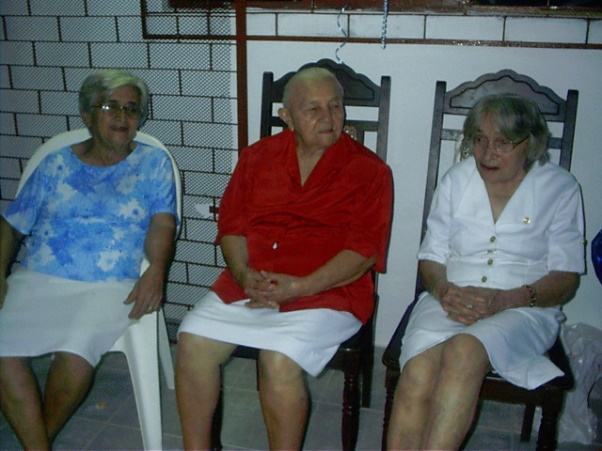
\includegraphics[width=2.72785in,height=2.04669in]{img/lourdes/image2.jpeg}

\begin{figure}
\centering
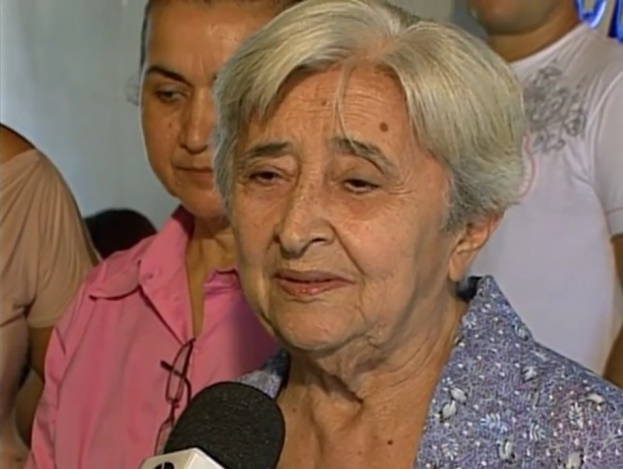
\includegraphics[width=4.49768in,height=2.13048in]{img/lourdes/image3.jpeg}
\caption{``Essa data é muito importante, porque comemora a Morte e a
Ressurreição de Jesus Cristo, que Ele Ressuscitou, Ele está Vivo aqui no
meio de nós, por isso tem Festa!'' -- Páscoa}
\end{figure}

\begin{figure}
\centering
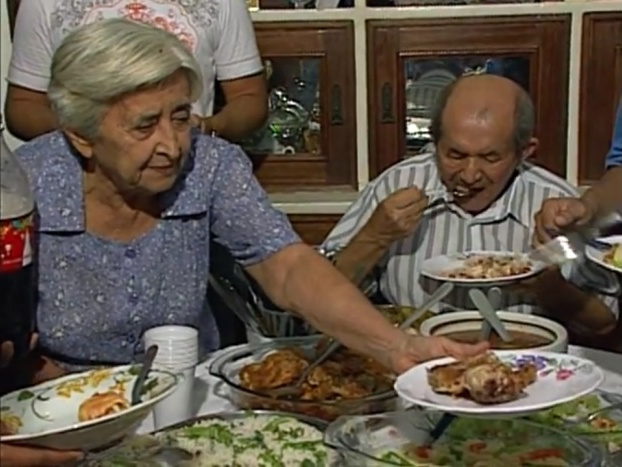
\includegraphics[width=4.47917in,height=2.12171in]{img/lourdes/image4.jpeg}
\caption{Tinha o maior prazer em SERVIR! Isto é AMAR -- AMAR É SERVIR!}
\end{figure}

\hypertarget{walter-pai}{%
\section{Walter (pai)}\label{walter-pai}}

pendente.

\hypertarget{fuxe1bio}{%
\section{Fábio}\label{fuxe1bio}}

Mamãe costumava de deixar na casa de vovó durante um tempo, nos meus
primeiros anos de vida. Quando cresci não podia deixar de ser diferente:
\emph{acertei a casa dela sozinho} e aparecia sempre para brincar com os
primos e colegas.

Vez por outra eu notava que vovó Maria vinha no muro brechar os netos,
demonstrando o cuidado e amor que tinha conosco.

Minha esposa Kelma e meu primeiro filho Fábio Lucas tiveram o prazer de
conhecê-la. Kelma, ainda hoje, lembra daqueles cabelos prateados,
saudades!

\hypertarget{walber}{%
\section{Walber}\label{walber}}

Uma das primeiras lembranças que tenho de vovó é dela me ensinando que
ela era minha segunda mãe. Eu devia ter uns 4 ou 5 anos de idade. Por
algum motivo eu fiquei na casa dela sem meus pais e ela me disse:
``\emph{Aqui também é sua casa. Você não tem sua mãe? Então! Eu sou a
mãe da sua mãe. Eu sou sua segunda mãe.}''

Tenho muitas lembranças de como minha avó era, lembro dela lendo a
bíblia comigo, com minha mãe e com vovô, em outras ocasiões lembro de
algumas poucas reclamações por leves travessuras que fazíamos, lembro
dela na cozinha de sua casa, lembro dela reclamando quando vovô queria
dar beijinhos nela na frente da gente em algumas comemorações e ela
demonstrava sua timidez. Mas sempre que me lembro dela, a primeira
imagem que quase sempre vejo é o sorriso estampado no seu rosto. Era
assim que ela sempre recebia a mim e a meus irmãos.

\hypertarget{wagner}{%
\section{Wagner}\label{wagner}}

Então.. vai aqui um breve relato (o que a memória me permitir) das
experiências que tive com vovó Maria.

Quase todas as vezes que vovó me encontrava, ela sempre me dizia que
\emph{quando eu era bebê, vovô fez uma caixa de madeira e forrou com
almofadas para me colocar dentro}. Ela dizia que ficava na cozinha
fazendo almoço e lavando a louça enquanto eu ficava nessa caixa em cima
da mesa da sala.

\begin{figure}
\centering
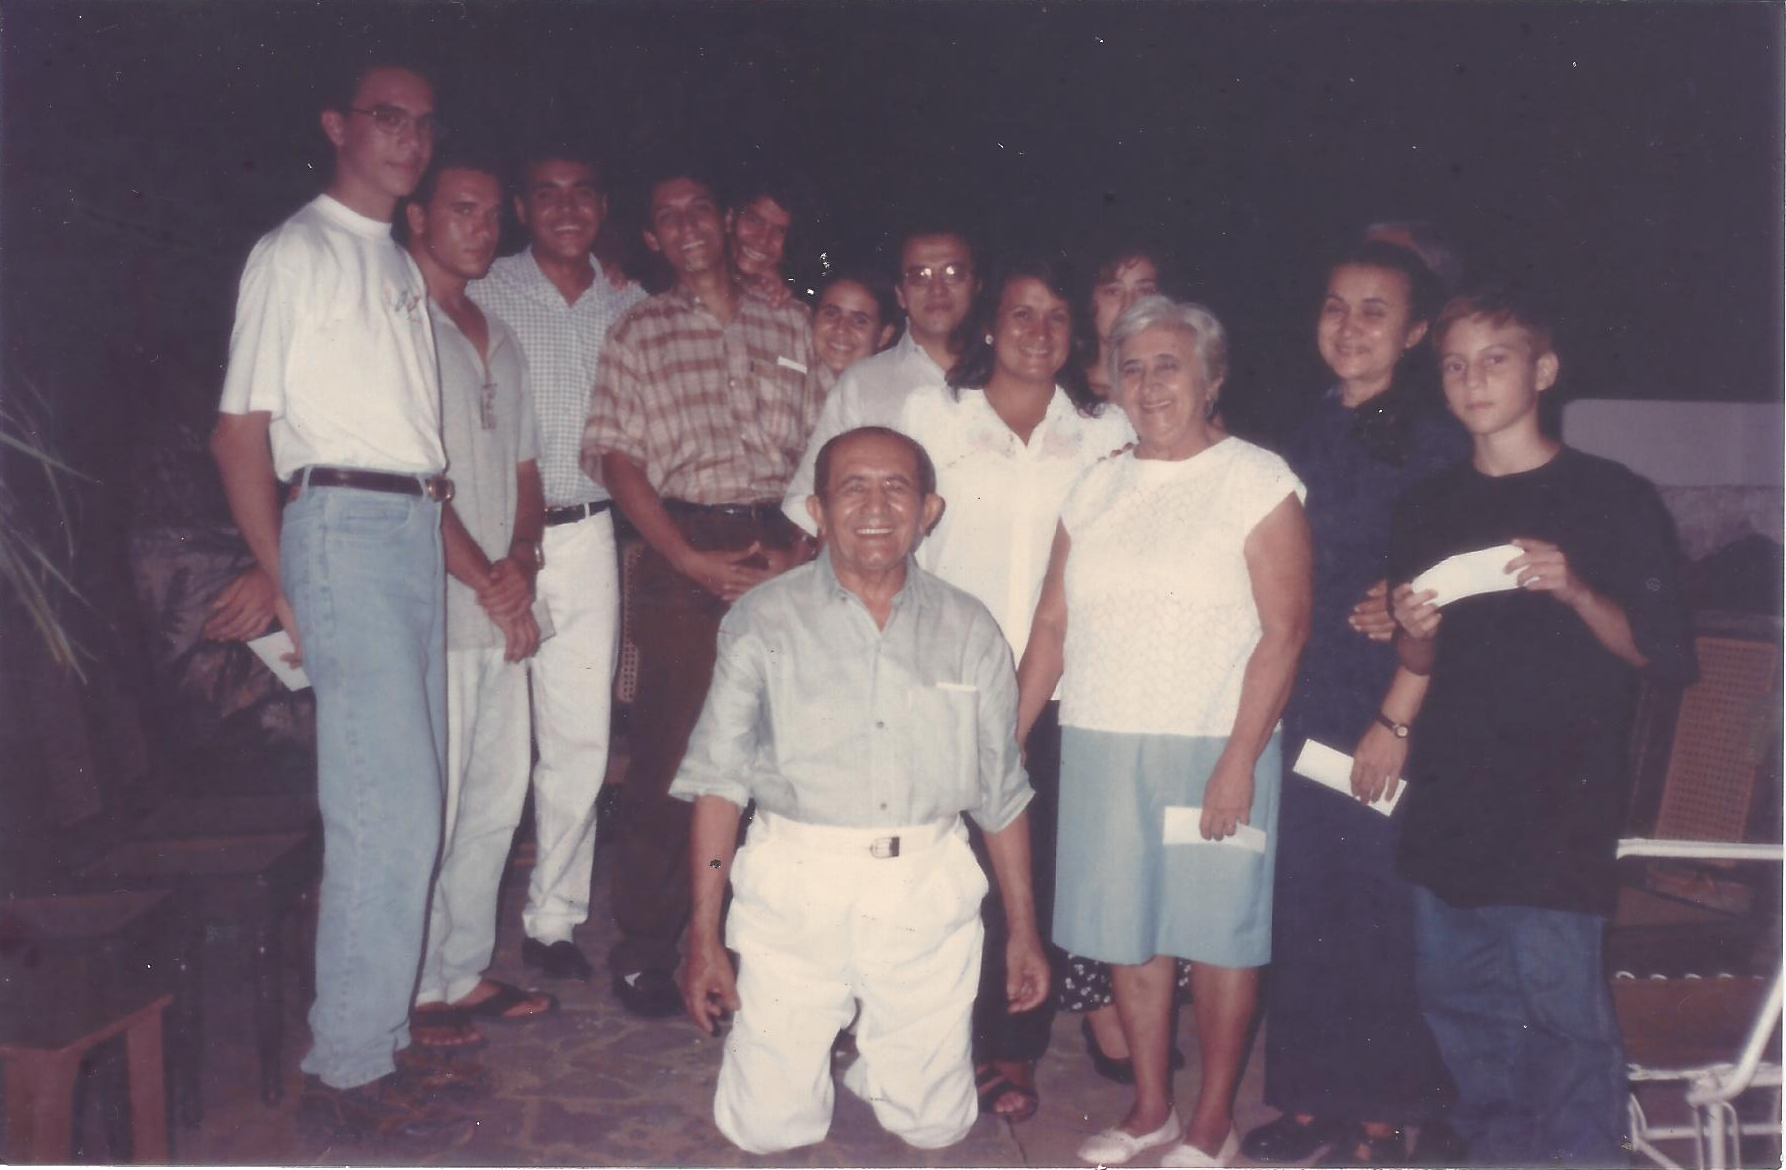
\includegraphics{img/dudu/wagner.png}
\caption{Vovó sempre nos recebeu com um belo sorriso, apesar de não
gostar muito das expressões de carinho de vovô em público. Era muito
vaidosa com seus cabelos (grisalhos).}
\end{figure}

Ela sempre me chamava para eu ir pegar ciriguela e jambo. Sempre, eu
subia no pé de jambo e passava horas lá. Quando descia, pegava um
ciscador, pá e vassoura para limpar o terreno (sempre caía folhas e os
caroços dos jambos que eu comia).

A ``santinha'', como chamava vovô, sempre falava que gostaria que a
gente (eu e meus irmãos) aparecesse mais lá.

Ela era uma mulher de fé. Sempre à via rezar e o terço sempre estava na
cômoda de seu quarto.

Por mais que a saudade venha de vez em quando mas eu sou prova de que o
amor da família a fez viver bem (na medida do possível). Mesmo nos
últimos dias de vida, com a voz baixinha e respiração curta, seu sorriso
brilhante era sempre sua recepção.

\hypertarget{famuxedlia-de-dora}{%
\chapter{Família de Dora}\label{famuxedlia-de-dora}}

\hypertarget{dora}{%
\section{Dora}\label{dora}}

\hypertarget{lembranuxe7as-de-minha-querida-muxe3ezinha-e-meu-pai-querido}{%
\subsection{Lembranças de minha querida mãezinha e meu pai
querido}\label{lembranuxe7as-de-minha-querida-muxe3ezinha-e-meu-pai-querido}}

\textbf{Pra falar de Maria, tem de falar de Pedro Santana eles eram
muito unidos}.

\begin{figure}
\centering
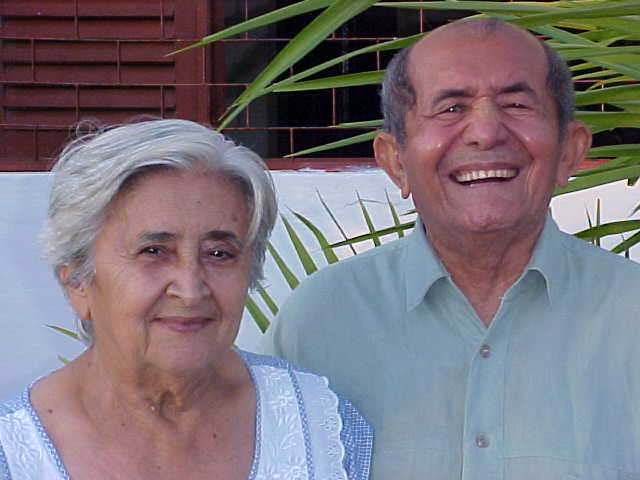
\includegraphics[width=1.5in,height=1.12519in]{img/dora/image1.jpg}
\caption{Papai e mamãe me faziam rir muito}
\end{figure}

\textbf{Um dia papai} chegou da feira e como era de costume trazia
presentes para mamãe, eu achava lindo o amor dele por ela, mas no final
queria sempre beijos e abraços e mamãe não queria, morria de vergonha.
Então num belo dia ele trouxe um \textbf{Pé de Coentro} bem bonito,
cheio e cheiroso eu estava por perto e ele chegou cantando e ficou de
joelhos e disse; \emph{Minha querida olha o presente que trouxe para
você}\ldots{}

Ela olhou pra ele e disse \emph{``Mas Pedro isso é presente''}? E fez um
gesto na boca e ele depressa se levantou e correu para abraça-la. Ela
recusou e ele disse \emph{Não vai me abraçar? Pois eu vou abraçar o Pé
de Jambo e vou dizer a todo mundo que perguntar `Por que Pedro tu estas
abraçado no Pé de Jambo?' e eu vou dizer `Maria não quer me abraçar'} e
saiu para o lado de fora e ficou agarrado no Pé de Jambo horas e eu
vendo aquela cena ri bastante, depois de muito tempo dela pedir pra ele
entrar e dizer \emph{``pronto eu deixo você me abraçar''} e ele saiu
correndo a dar cheiro e abraços nela e ela dizia ``\emph{sai Pedro, sai
Pedro}''\ldots{}

\textbf{Outro dia papai} começou a contar histórias da Bíblia pra os
vizinhos, e toda noite a nossa sala, na casa em Jaguaribe, ficava cheia
das pessoas querendo ouvir as belas histórias de papai que tinha um
jeito diferente de contar, por exemplo: Papai contava a história e
encenava os personagens sozinho, se na história ele dizia o homem
caiu\ldots{} ele caia de verdade, se dissesse o homem sorriu\ldots{} ele
dava belas gargalhadas e assim por diante. O público amava, e juntos, a
gente ria bastante, mas \textbf{D. Maria\ldots{}} não gostava de jeito
nenhum, dizia: ``\emph{Pedro não me mate de vergonha, pare com isso}'' e
ficava puxando a camisa dele e controlava a hora de terminar a nossa
animada noite de contação de histórias, e assim era os dias. Mamãe era
preocupada e não queria que ninguém reclamasse dele.

\textbf{Outro dia} arrumei um namorado e mamãe ficava na porta
assistindo a TV e vendo agente no terraço, então agente ficava
conversando e o namorado dizia baixinho ``Como a gente vai dar um
beijinho?''. Eu dizia ``\emph{Não tem como, mamãe esta de olho na
gente}''.

E de repente, \textbf{Mamãe} começou a cochilar e aproveitamos para dar
um selinho, \textbf{Supinpa!}. Mamãe como se fosse um raio levantou-se e
disse \emph{"Auxiliadora esta na hora de entrar kkkkk}``, e o namorado
disse''\emph{Como ela viu? Ela estava dormindo!}" kkkkkkk e assim era
\textbf{D. Maria} , eu disse a ele: "\emph{Foi uma armadilha e você
caiu, \textbf{Mamãe} se fez que estava dormindo e se preocupa muito
conosco e não aceita aproximação} e o namorado foi triste pra casa,
então \emph{Nosso namoro vai ser assim, sentado e somente conversar eu
disse vai sim, ai da gente se desobedecer a \textbf{D. Maria} kkkkkkkk}.

D. Maria gostava de fazer a feira e de escolher tudo a dedo, então outro
dia fomos eu, Lucia e ela pra o Mercado Central e no caminho Lúcia foi
pra outro local antes e \textbf{Mamãe disse:} \emph{Lúcia pare o carro,
você desviou do caminho, não é por aqui, tem de ir por aquela rua
kkkkkkk} Lúcia disse: \emph{``Mamãe eu vou para a Feira, mas antes eu
vou resolver um problema aqui''}. E as duas iam batendo boca porque
Mamãe não gostava de ser contrariada quando saia e dizia que Lúcia não
prestava atenção nas coisas. Na feira, ela já era esperada pelos
feirantes, eles a chamavam pelo nome, ``\emph{D. Maria o que a senhora
vai levar hoje? Eu guardei (verduras, carne, galinha etc\ldots), o
melhor para a senhora levar hoje!}'' E eu olhava aquela cena e ficava
feliz, porque Mamãe era muito séria, mas nestes momentos ela dava aquele
sorriso lindo que tinha. Uma das satisfações que eu sempre presenciava
era mamãe fazer compras, ela amava trazer tudo do bom e do melhor pra
todos nós em casa.

\textbf{Outro dia} eu arrumei meu 1º emprego foi num Banco eu era Caixa
e aquele emprego me deixava muito feliz porque eu queria ajudar em casa
nas despesas, Lúcia era contra queria que eu estudasse, mas eu terminei
convencendo \textbf{Mamãe} e assim fui trabalhar. Me lembro quando
ganhei meu primeiro salário, chequei em casa radiante e mostrei a
\textbf{Mamãe} a conta da \textbf{Energia e Água} que eu havia pago e
entregava o restante do dinheiro pra ela. Então ela disse, ``\emph{Venha
cá minha filha}'', e sentamos juntas. Ela pegou um lápis e caderno,
perguntou \emph{quanto eu gastava de passagem}, eu respondi, e ela
separou a quantia das passagens, depois disse: ``\emph{Esse restante
aqui você divide por 2, e com a metade abre uma poupança e a outra
metade compra suas necessidades, roupa, sapato}'' e eu disse \emph{``Mas
\textbf{mamãe}, eu quero ajudar em casa, e a senhora e papai\ldots{}''}
Então ela com aquele sorriso lindo disse: "\emph{Minha filha, você já
esta ajudando, pagou a conta de \textbf{Água e Luz} e agora já pode se
manter e comprar suas coisas, não precisa me dar mais nada}. Eu fiquei
sem jeito, porque não esperava aquela resposta, que complementou
dizendo: \emph{Você trabalhou o mês inteiro, é justo ficar com o fruto
do seu trabalho, ajudou em casa, vai guardar dinheiro e vai se manter,
parabéns"}. Eu saí feliz da vida com aquela divisão do meu 1º salario.

\hypertarget{jarbas}{%
\section{Jarbas}\label{jarbas}}

Pendente.

\hypertarget{daniel}{%
\section{Daniel}\label{daniel}}

A lembrança que tenho de vovó é que ela sempre foi muito caseira, as
vezes que ela veio lá em casa foi quando eu era pequeno -- recordações
só por foto mesmo -- mas tínhamos como rotina não só as festas e
comemorações em família mas também visitas frequentes para ver ela e
vovô. Em dias normais ela sempre estava ou na cozinha sentadinha
``vigiando'' algo no fogo com o rádio ligado, ou na sala na cabeceira da
mesa, se debruçando em alguma anotação, ela tinha um olhar um pouco
cansado, mas sempre nos recebia com um sorriso, e eu nunca abria mão de
dar um cheiro na cabecinha branca e cheirosa dela.

Sempre carinhosa com os netos e ranzinza com Tia Lúcia e vovô, cansei de
ver ela repreendendo Tia Lúcia com coisas do dia a dia e da casa, e vovô
sempre esperava ser servido por ela, que não só servia como ficava
pastorando vovô comendo, mais ainda quando ele já estava com problema na
visão. Nunca esqueço o tempero do feijão dela, simplesmente espetacular
seja do dia, ou requentado, o feijão diário caseiro pra mim era o
protagonista do prato, se fosse feijão com filé, me saboreava mais com o
feijão.

Nas festas de família ela sempre foi discreta, roupa só usava um modelo
de vestido que variava apenas a cor, e também sempre com os cabelos
cheirosos, como ela era pequena e a gente meio maior o cheiro na cabeça
branca era como um irmã, outras vezes um cheio na mão pedindo a bença a
ela. Infelizmente não lembro de uma conversa especifica que tivemos, mas
nos papos que mamãe tinha com ela, eu sempre opinava e na maioria das
vezes ela dava uns puxão de orelha em mamãe, ``Mais Dora\ldots{}''

Duas cenas me marcaram, quando ela estava no finzinho as filhas e ela
mesmo não queriam que ela fosse internada, e fui visitá-la. Ela estava
numa cadeira de balanço na cozinha ``agonizando'' com dores e
dificuldade para respirar, Tia Berna estava fazendo uma afago na cabeça
dela, fiquei indignado por ela não estar num médico, retruquei a todas
as tias para chamar uma ambulância sem sucesso, no mesmo dia ou no dia
seguinte veio a notícia, ela estava no Hospital da Unimed, corri pra lá
com mamãe e como fomos uns dos primeiros a chegar, junto com o pessoal
da funerária, e é um protocolo do hospital não dar auxílio algum na
remoção do corpo, então eu Luca e mamãe fomos onde estava o corpo dela.
Mamãe chorosa colocou uma roupa nela, ajeitou seus cabelos, e coube a
mim e a Luca colocar ela no caixão, foi meu último contato e lembrança,
não me recordo de nada do enterro e velório, mais sempre guardo a
lembrança de uma vovozinha afetuosa com todos a seu redor, que adorava a
casa cheia e sempre no comando da cozinha dava conta se todos estavam
servidos e satisfeitos.

Saudades de Vovó Maria!

\hypertarget{raquel}{%
\section{Raquel}\label{raquel}}

Vovó Maria sempre carinhosa e atenciosa com todos, sempre estava toda
arrumadinha e cheirosa.

Me lembro de uma tarde, quando ela estava internada no Memorial São
Francisco, eu fui lá para ficar com ela, aí quando mainha chegou pra me
render, vovó perguntou se podia pegar uma carona comigo pra casa (ela
não gostava de jeito nenhum de hospital e dizia que estava com saudade
da sua casa)\ldots{}

Aí eu disse \emph{``Mas vó eu to de moto''\ldots{}} aí ela respondeu:
\emph{mas você me leva de moto mesmo!} kkkkkkkk Eu e mainha não nos
aguentamos e sorrimos muito\ldots{} Expliquei a ela que naquele dia não
iria dar certo, mas que logo logo ela estaria em casa.

\hypertarget{rafael}{%
\section{Rafael}\label{rafael}}

No último ano em que Vovó Maria estava aqui entre nós, eu tinha apenas
13 anos, então como faz muito tempo e na época eu era bem dizer uma
criança ou adolescente, não tenho tanta história pra contar.

\begin{figure}
\centering
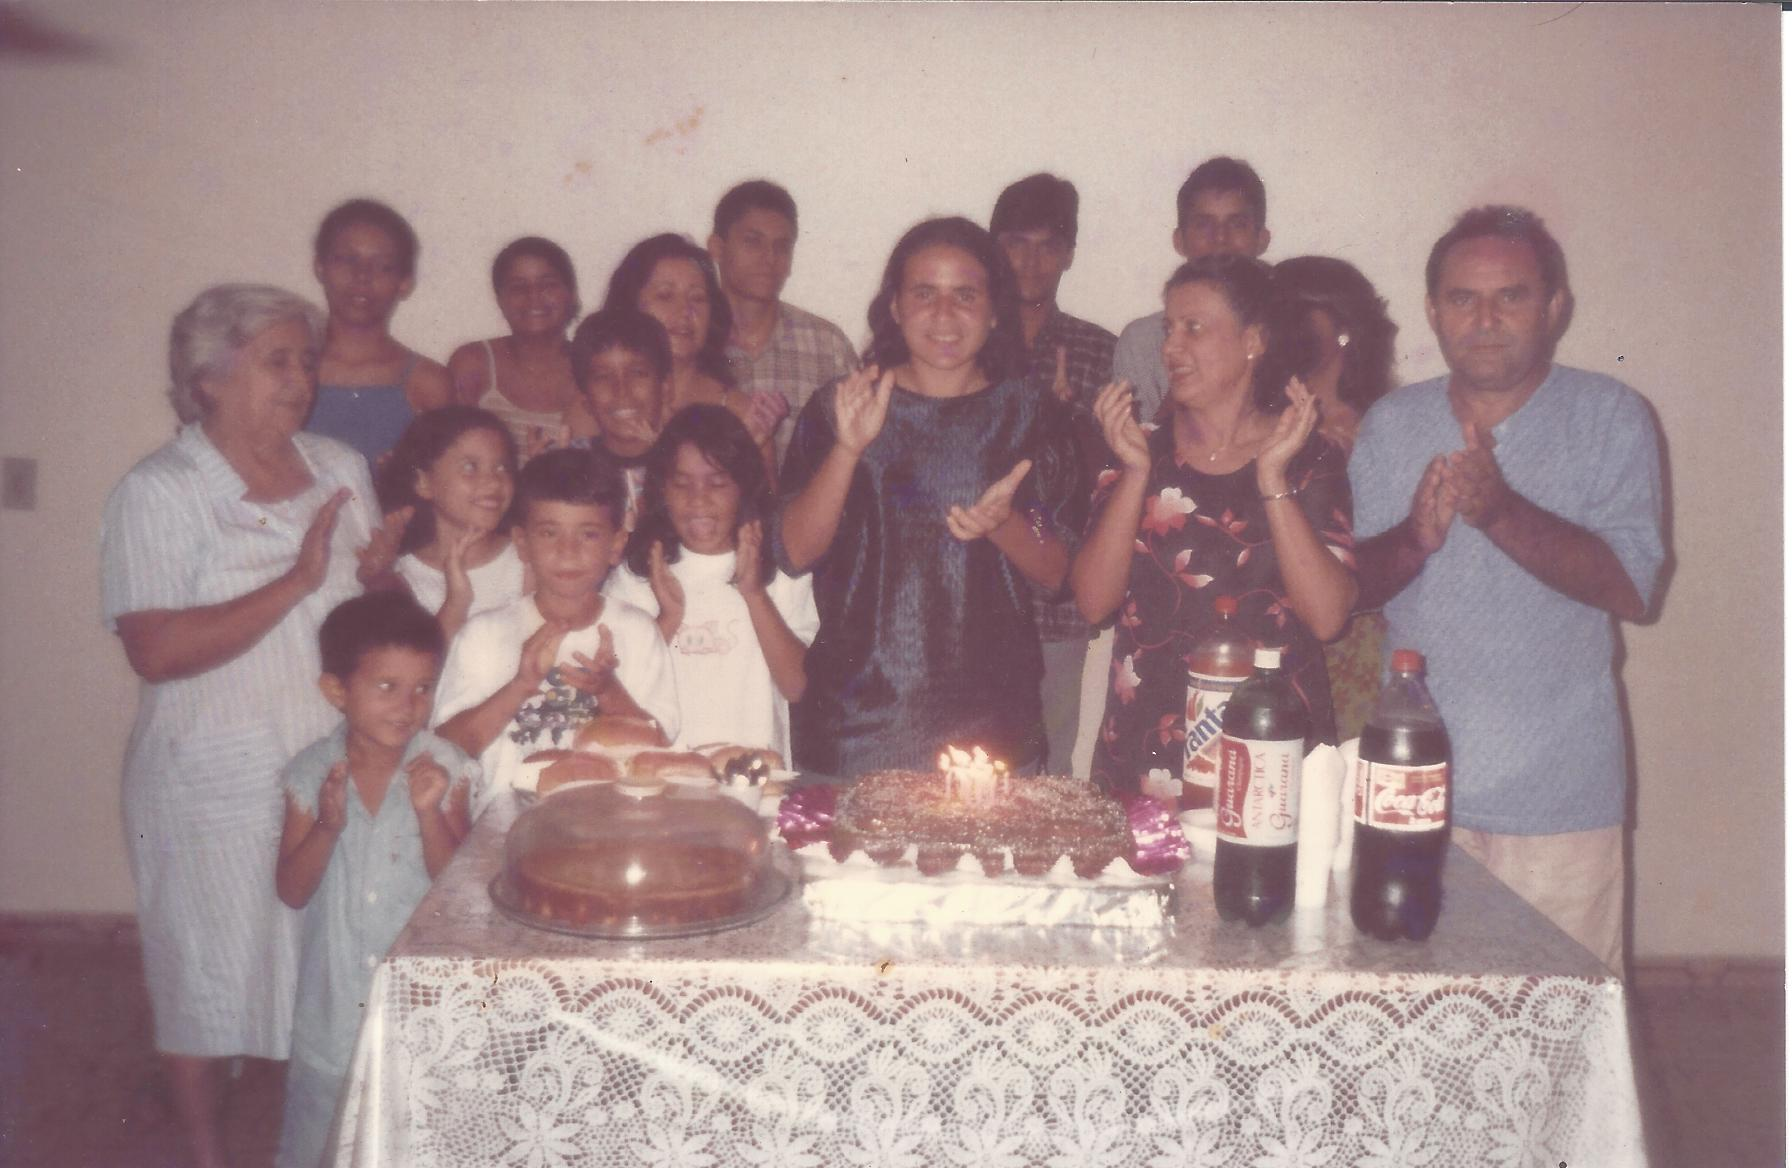
\includegraphics{img/dudu/vovo-festa-rafael.png}
\caption{Mesmo pequeno, não tenho como esquecer o quanto vovó gostava de
reunir a família.}
\end{figure}

Ela amava fazer o almoço e a sobremesa com muito amor e carinho pra
todos. Quando a família se reunia na casa dela em alguma data
comemorativa ou celebração cristã, que até os dias de hoje é tradição
ter sempre um almoço com todos da família, e ela sempre esperava que
todos colocassem seus pratos de comida, e fazia questão de ser a última,
pra garantir que todos se servissem bem.

Por fim, lembro-me o quanto vovó Pedro era carinhoso com ela (ele enchia
ela de beijos e abraços) mas ela era muito tímida, de poucas palavras ao
contrário de vovô. Vovó sempre foi uma pessoa muito simples e bastante
família!

\hypertarget{famuxedlia-de-marta}{%
\chapter{Família de Marta}\label{famuxedlia-de-marta}}

\hypertarget{marta}{%
\section{Marta}\label{marta}}

Sou Maria Marta, a quinta filha de Pedro e Maria. Segundo a Maria mãe,
todas as vezes que ela engravidava depois do segundo filho, que tinha
sido mulher, a Tecla Maria, ela sempre queria que nascesse um homem,
pois assim fecharia a fábrica, do jeito que começou, mas, que nada.
Nasceu outro homem, que infelizmente faleceu nos seus braços, depois
outra mulher, outra, e outra e finalmente, nasceu eu, na maternidade São
Vicente de Paulo, Jaguaribe, em João Pessoa, Pb. E, diga-se de passagem,
em berço de ouro, a melhor fase na vida dos nossos pais. Eu não lembro,
é claro, mas, dizia a Maria mãe, que Maria Marta era muito chorona e que
pra se ver um sorriso na minha boca, era coisa difícil demais\ldots{}
Talvez, por isso, hoje eu tenha o sorriso solto. Tentaram tanto me fazer
rir, que ficou na mente e hoje, eu rio atoa, rindo\ldots{}

Pois bem, estou aqui para falar de um momento especial com ela, Maria
mãe, que eu amo tanto. Tivemos um relacionamento muito tumultuado,
porque eu tinha um gênio que ela parecia não entender. A minha
curiosidade infinita a assustava e talvez por ela ter tantos filhos, não
dava tempo pra responder todos os meus questionamentos. Enfim, cresci e
chegou a hora de eu me afastar da família. Lembro do meu casamento como
se fosse hoje, eu não queria me casar vestida de noiva, mas, por ela,
fiz o sacrifício. Também não queria me casar de branco, mas, de tanto
que ela insistiu, eu mandei fazer um vestido branco e amarelo, da cor do
sol. Comprei o tecido e minha vizinha -- Ozita, amiga da família --
costurou e me deu de presente. Não queria fazer festa, mas, devido a
insistência da família, me organizei para receber os convidados no salão
da igreja. Pronto, tudo em ordem para o casamento acontecer e aconteceu.
Num dia de muita chuva e com atraso de uma hora do padre, enfim, nos
casamos.

Uma semana depois, viajamos pra Barra Bonita, São Paulo. Por seis meses
não nos falamos, só o Gilberto chegava com notícias, pois na época não
tínhamos telefone em casa. Naquele dia, eu acordei com muita vontade de
falar com todos e fui a uma cabine de telefone para fazer uma ligação.
Sim, naquela época, tínhamos que ir à telefônica para ligar para alguém,
porque até os orelhões, não faziam ligações para outro estado.

A lembrança que eu tenho desse dia é muito marcante. Quando a
telefonista passou a ligação para mim, minha mãe estava na linha e pela
primeira vez, tivemos uma conversa civilizada, rindo\ldots{} E naquele
dia ouvi da boca dela que sentia muitas saudades de mim, que a casa
tinha ficado vazia, que o meu sorriso, que alegrava a casa, estava
fazendo muita falta. Disse que meu cantar entoava em seus ouvidos e
tinha a sensação que eu sempre estava por perto e que ela já não dançava
mais com ninguém, risos\ldots{} (\emph{todos os dias que eu chegava da
escola eu ligava o rádio bem alto, agarrava ela e a fazia
dançar\ldots{}}). Enfim, pela primeira vez eu ouvia da minha mãe que eu
fazia falta para ela, e até hoje, esse momento me emociona. Pela
primeira vez me senti, verdadeiramente, amada. Ela me pediu perdão por
tantos momentos que poderíamos ter vivido intensamente e finalmente eu
percebi que ela apenas não tinha tempo pra mim e que ela também me
amava, só não tinha tempo para ficar falando, porque sempre tinha um
menor pra cuidar (depois de mim, mais duas mulheres e um homem).

Depois desse dia, nunca mais brigamos. Quando eu voltava a João Pessoa,
era sempre tão lindo\ldots{} Ela fazia tudo que eu gostava e o tempo
inteiro queria conversar, saber das minhas conquistas, etc. Desde a
nossa conversa que eu percebi e aprendi, que não precisamos ficar o
tempo inteiro falando do amor que sentimos, mas, precisamos dar
segurança a esse amor e levei como exemplo pra vida. Amar e falar que
ama. Quem quiser que saiba aproveitar o momento.

Se eu for falar dos belos momentos que vivemos juntas depois daquele
papo, acabaria escrevendo um livro, então, vou parando por aqui,
risos\ldots{}

\hypertarget{andruxe9a}{%
\section{Andréa}\label{andruxe9a}}

\hypertarget{memuxf3rias-com-vovuxf3-maria}{%
\subsection{Memórias com vovó
Maria}\label{memuxf3rias-com-vovuxf3-maria}}

Tem coisa mais gostosa do que os cheiros e sabores que nos lembram a
nossa infância? No meu caso, muitos deles me lembram minha amada vovó
Maria! Talvez por ter sido a neta distante, as comidinhas dela tenham me
marcado ainda mais, por fazerem parte de momentos raros e tão especiais
com meus avós e com a família toda. Toda vez que eu sinto cheiro de
coentro, vem imediatamente à mente, e ao coração, o rosto da nossa
Maria! Lembro daquele feijão com abóbora que só ela sabia fazer (apesar
de eu ter tentado muito fazer igual!). Ah, e a fritada? Que delícia, me
vem agora mesmo a vontade de comer e de dar um abraço na minha vovó!
Fora o manjar tricolor, que faz parte da história da família Santana!

A vovó Maria gostava de fotos e recordações de família como eu. Me
lembro de quando ela mostrou para mim e para o Ricardo -- que na época
era meu namorado e tinha ido conhecer a família -- os álbuns tão
queridos dela com fotos de todos\ldots{} e ela disse bem assim:
``\emph{um dia vai ter a foto do casamento de vocês dois aqui neste
álbum!}''. No dia da festa surpresa de casamento que a família fez para
nós, ela já estava enfeitando os céus com sua graça, mas eu senti a
presença dela, e às vezes quando tento me recordar daquela celebração
tão emocionante, parece que consigo ver o rostinho dela lá participando
com a gente\ldots{} E agora nossa foto está no álbum dela, como ela
tanto queria\ldots{}

Mas tem algo ainda mais profundo no meu vínculo com a minha avó Maria.
Toda vez que olho no espelho eu me lembro dela! Por um simples e lindo
motivo: ela me deixou uma preciosa herança, sua pinta acima da
sobrancelha esquerda! Uma vez eu falei para Tainá, minha filha, quando
ela tinha uns cinco anos: \emph{``Esta pinta aqui é da sua bisavó''}.
Eis que ela ficou intrigada e então me perguntou: \emph{``Ué, como
assim, mãe? Você tirou a pinta dela e colou em você?''}. Não foi
exatamente assim, mas sinto que carrego um pedacinho dela em mim, como a
Tainá imaginou na sua cabecinha pura de criança\ldots{} tenho imenso
orgulho desta pinta, até porque ela representa a origem de tudo. Me
lembro como se fosse agorinha o vovô Pedro nos contando de quando se
apaixonou pela vovó Maria, que tinha uma irmã muito parecida com ela. E
que o jeito que ele tinha de reconhecê-la era exatamente pela pinta! Uma
marquinha que representa, assim, as raízes desta família linda que eles
formaram\ldots{} de certa forma é também por causa desta pinta -- que
agora carrego com orgulho também no meu rosto -- que todos nós
existimos!

\hypertarget{gil-filho}{%
\section{Gil (filho)}\label{gil-filho}}

Avó Maria, me recordo de seu olhar sereno, do cheiro e da cor do seu
feijão, da salada de frutas deliciosa que ela sabia fazer. Sempre
cuidando de todos e sempre ao lado de vovô Pedro.

Tivemos poucas conversas longas, vezes por ser criança, vezes por ser
adolescente bobo, mas sempre levando alguma bronca por estar pendurado
em seu pé de jambo, inesquecível pé de jambo, que em todo natal ficava
repleto de luzes incandescentes coloridas para receber toda a família.

Me recordo desses natais, onde todos se sentavam ao redor do pé de jambo
e brincávamos na casa da vovó. Bons momentos. Sua energia se espalhou em
todos nós e ficamos com as saudades desses instantes felizes.

\hypertarget{famuxedlia-de-cristina}{%
\chapter{Família de Cristina}\label{famuxedlia-de-cristina}}

\hypertarget{cristina}{%
\section{Cristina}\label{cristina}}

Minha linda e amada Mamãe,

Cabelos cor de prata, impecavelmente penteados e finalizados com o creme
de pentear Kolene, sorriso acolhedor. No rosto, tinha a expressão do
amor, usava um hidratante da marca Pond`s e o Pó Compacto Promesa. Seu
cheirinho inesquecível de perfume Alfazema e sabonete Alma de Flores...
Gostava de após o banho colocar um talquinho de Alfazema. Tinha a fala
mansa, e amava cuidar da família. Essa foi a minha Mamãe.

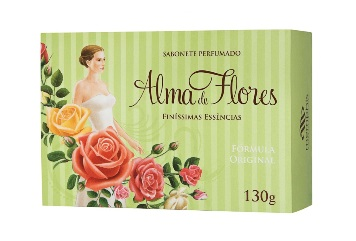
\includegraphics[width=1.60579in,height=1.08798in]{img/cristina/image1.jpeg}
\includegraphics[width=1.06181in,height=1.18458in]{img/cristina/image2.jpeg}
\includegraphics[width=1.175in,height=1.08773in]{img/cristina/image3.jpeg}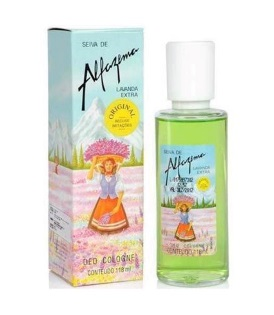
\includegraphics[width=1.22708in,height=1.41164in]{img/cristina/image4.jpeg}

Sou a caçula das 07 mulheres. Tive uma infância atormentada por crises
de asma. Recordo de ter tomado vários remédios, ``poções'' ensinadas
pelos mais antigos da família. O engraçado é que não podia revelar: ``Se
souber o que é, a asma volta''! O fato é que fui cuidada com todo amor e
hoje estou aqui, aos 57 anos, escrevendo esse relato...deu certo!
Hahaha.

Lembro de brincar com Feliciano de donos de casa, e os móveis eram
feitos com as embalagens de talco dela e caixinhas e fósforo. Tempo
bom...

Das coisas que minha mãe mais gostava, uma era ir à feira livre, e
cozinhar para toda família. Que saudades sinto da sua comidinha, dos
almoços de fim de semana, do cozido mais delicioso do mundo! Era a
última a sentar na mesa. Queria ter a certeza que todos estavam bem
servidos. Nas Ceias Natalinas, ela preparava uma galinha de forno, minha
nossa! Dá água na boca só de lembrar... rs. Não era permitido tocar na
comida até que todos estivessem presentes e que fosse feita a oração.
Ah, minha mãe, saudade desses momentos...

Me casei muito jovem, aos 16 anos, e ainda por cima grávida. Nunca me
recriminou por isso, pelo contrário. O que ela me disse foi: ``De
criança eu sei que você sabe cuidar, será uma boa Mãe. Casamento não é
fácil, minha filha, e você não irá para a sua casa. Faça por onde
viver''. Fui morar em Campina Grande após 2 anos e 07 meses morando com
a minha sogra. As dúvidas que tinha para cozinhar, ligava para ela, que
descrevia em detalhes como fazer um delicioso feijão. Porém, por mais
que eu tentasse, nunca consegui alcançar o mesmo sabor do feijão e da
carne. Lembro de nossas conversas quando precisava de conselhos, e a
carninha guisada sempre à espera no forno para comer com pão francês.
Que delíciaaaaa...

Na festa de seus 50 anos de casada, cheguei mais cedo para ajudá-la a se
arrumar. Perguntei se podia maquiá-la, ela disse: ``hoje eu quero tudo
que tiver direito!'' No rosto, o pó de arroz Promesa e um pouco de
rouge. Na boca, um batom rosa clarinho. As unhas, permitiu pintar com um
rosa bem clarinho também. A roupa era um conjunto e saia e blusa azul
claro. Estava pronta e sorridente a nossa Rainha para entrar na Igreja
com seu Rei. Foi uma cerimônia linda e o jantar com familiares e amigos
em sua casa. Como estavam felizes aquela noite! Essa foto abaixo, foi
quando fizeram 62 anos de casados: chegamos lá com o buquê e a mensagem
assinada pelos filhos. As fotos dizem tudo:

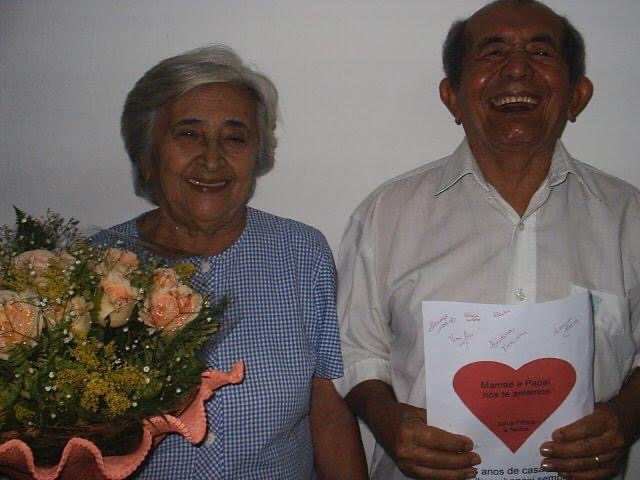
\includegraphics[width=2.73889in,height=2.05417in]{img/cristina/image5.jpeg}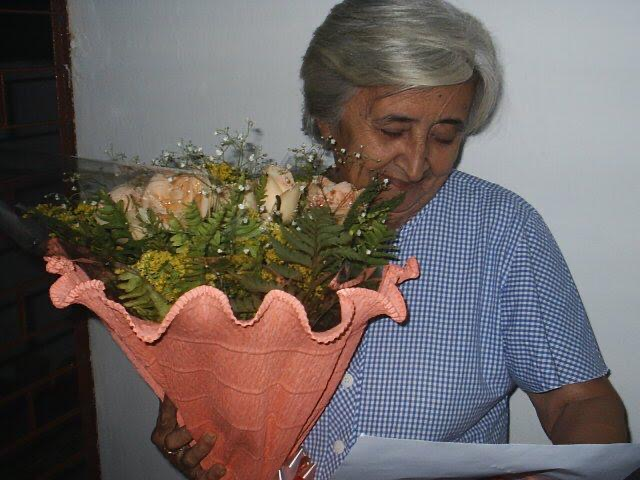
\includegraphics[width=2.72917in,height=2.04687in]{img/cristina/image6.jpeg}

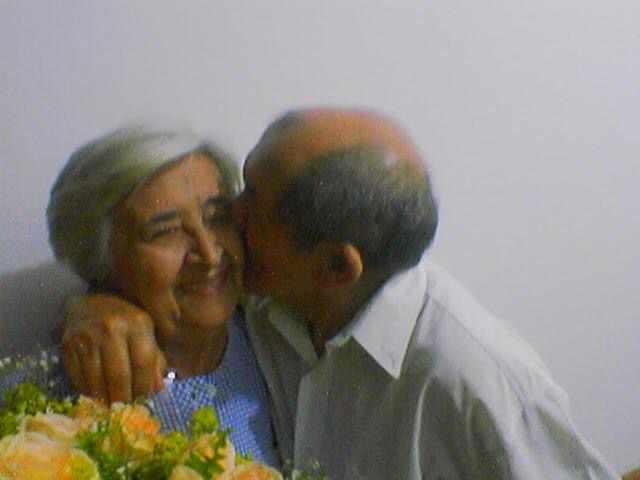
\includegraphics[width=2.73889in,height=2.05417in]{img/cristina/image7.jpeg}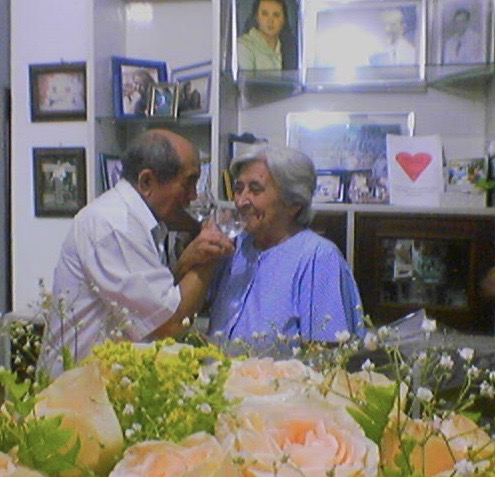
\includegraphics[width=2.13961in,height=2.06181in]{img/cristina/image8.jpeg}

Eu achava a coisa mais linda eles na missa. Tinham lugar cativo na
Igreja, e ao final sempre abraçava a todos. Nos revezávamos para
buscá-los e tenho na memória a imagem deles saindo de mãos dadas, mamãe
com todo cuidado para que papai não esbarrasse em nada. Foi uma mulher
guerreira, batalhou muito com papai. Mulher sábia, tímida, era de falar
pouco, mas esse pouco era o que precisávamos ouvir. Amava quando ligava
pra mim dizendo: ``Minha filha, tem um cozidinho aqui, você quer?'', e
eu, mesmo que já tivesse almoçado, ia lá correndo só para experimentar
aquela comida tão saborosa e feita com tanto amor.

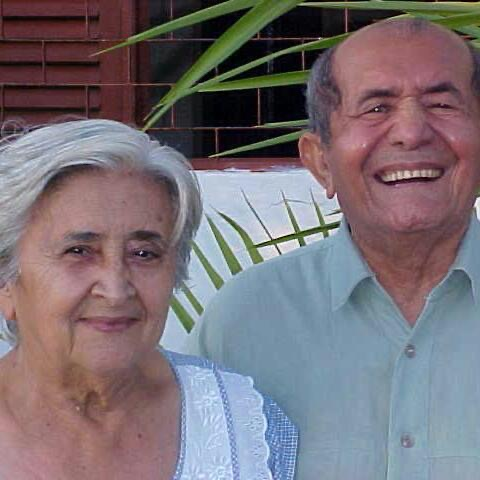
\includegraphics[width=1.96875in,height=1.96875in]{img/cristina/image9.jpeg}

Minha Mãe, como sou grata a Deus por ser sua filha. Assim como Papai, a
senhora deixou uma herança linda, não de bens materiais, mas o mais
valioso de todos, O EXEMPLO! São tantas lembranças com a senhora que vem
na memória que não daria aqui para transcrever. Só sei que hoje, quando
lembro da senhora, pareço sentir seu cheiro e o toque de seus cabelos em
minhas mãos. Guardo tudo dentro do meu coração.

Minha Mãe, minha Maria no Céu, meu exemplo de Amor e dedicação.

Te amo para sempre.

Sua caçula Cristina.

\hypertarget{victor}{%
\section{Victor}\label{victor}}

pendente.

\hypertarget{famuxedlia-de-feliciano}{%
\chapter{Família de Feliciano}\label{famuxedlia-de-feliciano}}

\hypertarget{feliciano}{%
\section{Feliciano}\label{feliciano}}

\hypertarget{uma-muxe3e-incomparuxe1vel}{%
\subsection{Uma Mãe Incomparável}\label{uma-muxe3e-incomparuxe1vel}}

"Eu sou Feliciano Santana de Jesus\ldots{} Nascido em nove de Junho de
1965, na Maternidade São Vicente de Paula, João Pessoa-PB. Filho de
Maria José de Santana e Pedro José de Santana.

Vou aqui, buscar em minhas memórias e meu coração, onde mantenho meu Pai
e minha Mãe, e o farei até o fim dos meus dias aqui na Terra.

Em minhas lembranças de mamãe, elas começam na Alberto de Brito --
Jaguaribe. Ali, eu lembro que mamãe sempre nos reunia no almoço em uma
mesa grande, e que as vezes eu gostava de passear por baixo da mesa,
coisa de menino pequeno mesmo! Lembro também de uma situação em que
mamãe, sempre abria um Cofre que Papai possuía e eu dizia a mamãe que
descobriria o segredo. Então como dito, eu usei um arame em um pequeno
orifício que havia na giratória do segredo, então a cada passo que o
arame percorria, eu dava uma volta contrária e assim, acabei descobrindo
o segredo! Quando eu disse a mamãe que sabia abrir, ela ficou surpresa!
E pediu para que eu abrisse. Eu bem orgulhoso do feito, abri e disse a
ele como havia feito. Então daquele dia em diante, provavelmente ela
comentou com Papai e ai eles não confiaram mais no cofre, pois se eu,
uma simples criança na faixa dos 7 anos consegui fazer tal façanha,
imagine um adulto!

Agente foi morar na Rua Severino Patrício, que fica na Torre, neste
local, lembro que mamãe me pedia para ir fazer o jogo do Bicho !, ela
gostava de fazer uma fezinha, nesse tipo de jogo, eu criança e gostava
de desafios e ao mesmo tempo descobrir os arredores, ia correndo lá na
venda de Dna Báia, era assim que eu a conhecia, lá eu levava as
anotações de mamãe e vez por outra ia buscar uns trocados quando ela
ganhava !, Mamãe sempre foi simples, e magnífica em tudo !, ali ela me
fazia ganhar confiança em mim mesmo, pois eu ia sozinho lá do outro lado
da pista onde passavam ônibus e carros, mas as instruções do trajeto,
mamãe, dizia, e eu seguia a risca ! e assim, sempre ia e voltava com
segurança. Mamãe, sempre Dna de casa de 1a qualidade, pois cuidava de
nós, eu e as meninas, e deixava tudo organizado, o amor de mamãe sempre
foi imenso !, e eu sempre a via com sorriso no rosto, mesmo sem sorrir,
parecia sempre serena.

Foi então que um belo dia, Bernadete e Duquinha, deve ter encorajado
mamãe a me levar para São Paulo, para fazer uma cirurgia de garganta de
lobo ! ( na verdade fissura labial interna) era uma fenda no céu de
minha boca, e lá eu fui operado no Hospital das Clínicas de São Paulo.
Pense ! mamãe e eu viajamos de avião até lá ! e lembro como hoje !, ao
abrir a porta dianteira do avião, minhas pernas tremeram na mesma hora
com o frio !, ainda bem que no dia em que chegamos, foi o ultimo dia de
inverno. Passamos 1 ano lá e eu gostava muito de poder conhecer uma
grande cidade como São Paulo com cerca de 9 anos de idade e voltei com
10 anos. Os finais de semana, Bernadete e Raimundo, ou apenas Bernadete,
sempre arranjava lugares para agente ir e conhecer essa grandiosa cidade
e quando fica sem sair, eu andava nos arredores, onde agente digamos,
morava !, no Largo 13 em Santo Amaro, enfim, voltei de São Paulo com a
garganta resolvida então, passei a viajar com Dora e as vezes com Papai,
para recife, toda semana, pois eu precisava fazer fonoaudiologia, para
aprender a falar corretamente, pois até então eu falei errado até os 10
anos de idade, fiz esse percurso por 2 anos seguidos. de volta, eu
comecei a estudar no Pio X, já me vestia sozinho, e quando saía de casa,
lembro sempre o "``Deus lhe acompanhe meu filho''", palavras de mamãe
para que o anjo da guarda me levasse e trouxesse em segurança. Eu nunca
me perdi no caminho. Os anos se passavam, eu crescia, terminei minha
oitava série, fui para escola Técnica, meu caminho diário era longo, as
vezes passa o dia na escola e mamãe sempre ali, conduzindo, orientando,
passei para universidade, mas eu estudava longe em Goiana-PE, chegava em
casa 11hs da noite e mamãe estava lá esperando eu chegar !. Essas coisas
sempre foram marcantes, muitas delas eu pedia pra ela não precisar
esperar, deveria dormir, descansar ! mas ai ela falava que só conseguia
dormir quando eu chegasse, coisa de mãe mesmo, são atitudes que um filho
nunca esquece na vida, terminei meu curso, trabalhei em alguns lugares
mas acabei criando meu próprio negócio, casei e tive 2 filhos, minha
felicidade, foi ver meu filho Pedro, recém nascido, nos braços de mamãe,
ali eu via a felicidade no gesto de ter ele novinho, poder esta r com
ele ali e isso me orgulhou de mais e emocionou muito, ela esteve no
Batizado dele com Papai e foi uma festa !, filmei tudo e bati várias
fotos, algumas vezes ela veio me visitar, eu morava no Bessa, mas a
maioria eu todo domingo ia pra casa dela, passava o dia lá, mas em
determinado momento, precisei me mudar para CG, pois Márcia havia
passado no concurso do BB e tivemos que nos mudar para RN, onde passei 2
anos e meio. um grande momento foi as Bodas de ouro de Papai e Mamãe,
uma festa magnífica e marcante para nós os filhos, pessoas da família,
amigos e amigas de Mamãe tiveram presente, agente fazia festa do dia das
Mães e era só alegria, mas eu aqui, mesmo tendo tantas coisas para
dizer, me reservo de não prosseguir, pois quero guardar comigo e passar
aos meus filhos, como a avó deles, Maria José de Santana, foi uma mulher
iluminada, exemplar, uma fortaleza de Mãe, uma Avó para eles, humilde,
simples, conselheira, com um sorriso de mãe para minha vida toda
lembrar, é aqui que desejo para com minhas palavras, desculpem, mas só
quero ter em meu coração o que já tenho, o Falecimento de mamãe, mexeu
com as estruturas de todos nós, mas essa parte, em diante, deixo nas
mãos de Deus ! este sim, a tem consigo !, tenho certeza, junto com meu
Pai Pedro José de Santana e meu irmão José Santana de Jesus. Obrigado
por fazerem essa Homenagem, obrigado por ela ter sido nossa mãe e sempre
será claro ! finalizo aqui minhas palavras e mantenho toda uma vida de
convivência, deste filho dela, em meu coração.

Feliciano Santana de Jesus

João Pessoa, 04 de junho de 2020

\hypertarget{muxe1rcia}{%
\section{Márcia}\label{muxe1rcia}}

\hypertarget{doce-maria}{%
\subsection{Doce Maria}\label{doce-maria}}

Venho por meio destas falar um pouco sobre minha sogra Dona Maria José
de Santana.

Transmitia uma tranquilidade no seu falar e no seu agir.

Das vezes que tive a feliz oportunidade de conversar com ela, percebia a
doçura em sua voz e às vezes falava tão baixinho que não conseguia
ouvi-la e a pedia para repetir.

Tinha grande empatia para com o próximo, independentemente de ser ou não
da família, e isso, na minha opinião, de certa forma,a deixava triste
por não poder ajudar.

Não diferenciava o amor pelos filhos mas, como sou a esposa de
Feliciano, não economizava ao falar do seu filho para comigo, falando do
amor que tinha por ele.

Quando morávamos em uma residência próxima a sua casa, toda semana, ao
fazer sua feira semanal, no Mercado Central, levava uma feira para nós
também e, por saber que Feliciano gostava do seu tempero, especialmente
do da carne, levava-a já temperada.

Não raramente, cheguei a vê-la com dor de cabeça, geralmente no final da
tarde.

Como a minha ida em sua casa era geralmente aos finais de semana,
presenciei algumas vezes ela sentada na sala de estar, assistindo Raul
Gil entre um cochilo e outro, alí mesmo naquela cadeira. Posteriormente
vim a saber por Lúcia, que os cochilos que dava durante o dia, eram
reflexos de uma noite mal dormida, me salvo engano, devido a uma tosse.

Eu achava interessante seu almoço, feijão com farinha e de sobremesa uma
laranja.

Gostava de jogar jogo do bicho o qual, ouvia o resultado por um rádio de
pilha que possuía e que ficava na cozinha. Ocorreu dela me explicar como
funcionava o jogo do bicho mas, eu nunca consegui entender.

Quando já enferma, cheguei a sua casa e a encontrei deitada em sua cama
e, conversando com ela, me confessou estar envergonhada por ter tentado
ir ao banheiro e não ter dado tempo, deixando o corredor sujo e, estar
dando trabalho as meninas o que estava a deixando triste por estar
passando pela aquela situação.

Exemplo de pessoa, sempre me tratou muito bem, com atenção, carinho e
tenho muito a agradecer a Deus por tê-la conhecido.

\hypertarget{famuxedlia-de-nezinho-irmuxe3o}{%
\chapter{Família de Nezinho
(irmão)}\label{famuxedlia-de-nezinho-irmuxe3o}}

\hypertarget{benedita-de-almeida-andrade-sobrinha}{%
\section{Benedita de Almeida Andrade
(Sobrinha)}\label{benedita-de-almeida-andrade-sobrinha}}

Tia Maria, era uma mulher que eu admirava muito, em tudo que fazia; era
organizada, sabia fazer coisas diferentes, e tinha prazer pelo que
fazia. Muito presente com a família e na vida dos filhos. Estou hoje com
76 anos!

\hypertarget{penhinha}{%
\section{Penhinha}\label{penhinha}}

\textless!Maria da Penha Almeida Bernardo (Sobrinha)--\textgreater{}

Tia Maria era uma pessoa muito alegre, sempre com um sorriso nos lábios,
nunca a vi triste. Achava-a muito bonita, tanto fisicamente como
espiritualmente. Era muito religiosa, tinha sempre uma palavra de
conforto. O nosso contato com ela era mais por telefone, as vezes que ia
lá era com Benedita e éramos muito bem recebidas! Ela fazia questão de
nos oferecer um ótimo lanche!. Na última vez que estivemos na casa dela.
Ela me deu uma foto dela com o tio Pedro e uma que tem as filhas, aquela
que tem todas as Marias!

O que mim faz lembrar dela é quando está chegando a Páscoa. Porque ela
nos convidou para participarmos da Páscoa junto com ela e a família.
Mas, no ato do convite ela falou : - Estou convidando, mas sei que vocês
não veem devido a distancia. E de fato, não fomos, não me lembro porque
deixamos de ir, era como se fosse uma despedida. Essa foi à última
Pascoa dela conosco.

\hypertarget{famuxedlia-de-jouxe3o-irmuxe3o}{%
\chapter{Família de João (Irmão)}\label{famuxedlia-de-jouxe3o-irmuxe3o}}

\hypertarget{silvia-almeida}{%
\section{Silvia Almeida}\label{silvia-almeida}}

Minha tia, a única coisa que posso falar, minha tia era um doce! Ela não
era mãe, era um doce de mãe pra vocês! Aquela maneira calma pra vocês,
aquela maneira tranquila, amorosa, maravilhosa! Ela é nota dez, dez,
dez! Tinha bons modos de falar com padrinho Pedro, era um casal
assim\ldots{} Meu Deus do Céu! Ela quando chegava na casa de vovó ,
chegava com aquele jeitinho dela: -- \emph{Bença mãe, como é que tá
mãe}? Era assim, a maneira que eu posso falar da tia Maria! A tia Maria
era Bênção do Senhor! Foi uma mãe dedicada a cada uma de vocês! Eu nunca
vi a minha tia falar alto, era muito educada. É tanta coisa maravilhosa
dela! Eu achava lindo quando eu chegava lá e ela estava fazendo bolo
para padrinho Pedro sair, e ele colocava dentro dos tabuleiro e colocava
dentro do carro e ela tinha aquela paciência. Era uma mulher que, os
dois né, era uma alma num corpo só!

Eu amo a cada um de vocês! Podia o mundo tá pegando fogo, mas a tia
Maria era aquela tranquilidade, vamos se acalmar. Quando chegava lá na
casa de vovó perguntava: -- \emph{Como é que tá Terna? Como é que tá
Augusta? Vocês estão bem}? Essa era a maneira dela falar, era com
carinho. Eu nunca vi a tia Maria se estressar! Eu nunca vi a minha tia
falar alto! Eu nem sei meu Deus do Céu, o que falar da minha tia! Eu
vejo em vocês primas e o próprio Duquinha, todos vocês doce! Mas a tia,
gente, eu nem sei mais o que vou falar sobre ela. Por ter sido uma
pessoa tão maravilhosa! São muitos predicados lindos dela, é a única
coisa que tenho pra falar acerca da minha tia, irmã do meu pai. Eu tenho
orgulho!

\hypertarget{amigos}{%
\chapter{Amigos}\label{amigos}}

\hypertarget{samira}{%
\section{Samira}\label{samira}}

\hypertarget{uma-palavra-um-conforto}{%
\subsection{Uma palavra, um conforto}\label{uma-palavra-um-conforto}}

Conheci Dona Maria através do seu neto Eduardo (Dudu), que também me
apresentou ao Senhor Pedro, marido de Dona Maria, ambos pessoas de Deus,
que durante anos fizeram diferença em minha vida, rezando por mim quase
que diariamente. Na ocasião em que conheci Dona Maria eu passava por
alguns problemas de saúde física e mental, e fui em busca de um alento
para minhas dores. Sempre tranquila e serena, Dona Maria, em um dia, dos
muitos que estive em sua casa, me confortou com uma palavra bíblica
seguida de uma oração. Seu olhar naquele momento me lembrou o da mãe de
Jesus, que ampara um filho no momento de tristeza. Depois daquele dia
senti uma paz que excede todo entendimento. Dona Maria me confortou, me
amparou, me tranquilizou e a ela sou grata até hoje.

\backmatter
\end{document}
